\section{Group Actions}

\subsection{Group Actions and Permutation Representations}

Let $G$ be a group and let $A$ be a nonempty set.

\begin{problems}
    \item Let $G$ act on the set $A$. Prove that if $a,b \in A$ and $b = g \cdot a$ for some $g \in G$, then \(G_b = g G_a g^{-1}\) (\(G_a\) is the stabilizer of $a$). Deduce that if $G$ acts transitively on $A$ then the kernel of the action is
    \[\bigcap_{g \in G} g G_a g^{-1}.\]
    \begin{sol}
		Suppose $h \in G_b$. We want to show that $h \in gG_ag\inv$. Since $h \in G_b$, we have $h \cdot b = b$. But $b = g \cdot a$, so $h \cdot (g \cdot a) = g \cdot a$. Applying $g\inv$ to both sides, we get $g\inv h g \cdot a = a$. This means that $g\inv h g \in G_a$, so $h \in g G_a g\inv$. Thus, we have shown that \(G_b \subseteq g G_a g^{-1}\). For the other direction, suppose $h \in g G_a g^{-1}$. Then there exists some $k \in G_a$ such that $h = g k g^{-1}$. We want to show that $h \in G_b$. We have $h \cdot b = (g k g^{-1}) \cdot (g \cdot a) = g \cdot (k \cdot a) = g \cdot a = b$, since $k \in G_a$ implies $k \cdot a = a$. Thus, $h \in G_b$. Therefore, we have shown that \(g G_a g^{-1} \subseteq G_b\). Combining both inclusions, we conclude that \(G_b = g G_a g^{-1}\).

		Now, if $G$ acts transitively on $A$, then for any $b \in A$, there exists some $g \in G$ such that $b = g \cdot a$. From the first part, we have \(G_b = g G_a g^{-1}\). The kernel of the action is the intersection of all stabilizers \(G_b\) for \(b \in A\). Therefore, the kernel is
		\[\bigcap_{b \in A} G_b = \bigcap_{g \in G} g G_a g^{-1}. \qh\]
	\end{sol}
    \item Let $G$ be a permutation group on the set $A$ (i.e., \(G \leq S_A\)), let \(\sigma \in G\) and let \(a \in A\). Prove that \(\sigma G_a \sigma^{-1} = G_{\sigma(a)}\). Deduce that if $G$ acts transitively on $A$ then 
    \[\bigcap_{\sigma \in G} \sigma G_a \sigma^{-1} = 1.\]
    \begin{sol}
		Suppose $\tau \in \sigma G_a\sigma\inv$. We want to show that $\tau \in G_{\sigma(a)}$. Since $\tau \in \sigma G_a \sigma^{-1}$, there exists some $\rho \in G_a$ such that $\tau = \sigma \rho \sigma^{-1}$. We have $\tau \cdot \sigma(a) = (\sigma \rho \sigma^{-1}) \cdot \sigma(a) = \sigma \cdot (\rho \cdot a) = \sigma(a)$, since $\rho \in G_a$ implies $\rho \cdot a = a$. Thus, $\tau \in G_{\sigma(a)}$. Therefore, we have shown that \(\sigma G_a \sigma^{-1} \subseteq G_{\sigma(a)}\). For the other direction, suppose $\tau \in G_{\sigma(a)}$. We want to show that $\tau \in \sigma G_a \sigma^{-1}$. We have $\tau \cdot \sigma(a) = \sigma(a)$. Applying $\sigma^{-1}$ to both sides, we get $\sigma^{-1} \tau \sigma \cdot a = a$. This means that $\sigma^{-1} \tau \sigma \in G_a$, so $\tau \in \sigma G_a \sigma^{-1}$. Thus, we have shown that \(G_{\sigma(a)} \subseteq \sigma G_a \sigma^{-1}\). Combining both inclusions, we conclude that \(\sigma G_a \sigma^{-1} = G_{\sigma(a)}\).

		Now, if $G$ acts transitively on $A$, then for any $b \in A$, there exists some $\sigma \in G$ such that $b = \sigma(a)$. From the first part, we have \(\sigma G_a \sigma^{-1} = G_b\). The kernel of the action is the intersection of all stabilizers \(G_b\) for \(b \in A\). Therefore, the kernel is
		\[\bigcap_{b \in A} G_b = \bigcap_{\sigma \in G} \sigma G_a \sigma^{-1} = 1. \qh\]
	\end{sol}
    \item Assume that $G$ is an abelian, transitive subgroup of $S_A$. Show that \(\sigma(a) \neq a\) for all \(\sigma \in G - \{1\}\) and all \(a \in A\). Deduce that \(|G| = |A|\). [Use the preceding exercise.]
    \begin{sol}
		Since $G$ is abelian, then the conjugate of $G_a$ is trivial, i.e., $\sigma G_a \sigma\inv = G_a$ for all $\sigma \in G$. From the previous exercise, we know that the kernel of this action is trivial. However, the intersection of all $\sigma G_a\sigma\inv$ is just $G_a$ so that $G_a = 1$. Then $G_a$ is trivial for every $a \in A$, hence $\sigma(a) \neq a$ for all $\sigma \in G - \{1\}$ and all $a \in A$. It follows by Proposition 4.2 that $|G|/|G_a| = |A|$, hence $|G| = |A|$ because $G_a$ is trivial.
	\end{sol}
    \item Let \(S_3\) act on the set \(\Omega\) of ordered pairs \(\{(i,j) \mid 1 \le i,j \le 3\}\) by \(\sigma((i,j)) = (\sigma(i), \sigma(j))\). Find the orbits of \(S_3\) on \(\Omega\). For each \(\sigma \in S_3\) find the cycle decomposition of \(\sigma\) under this action (i.e., find its cycle decomposition when \(\sigma\) is considered as an element of \(S_9\)—first fix a labeling of these nine ordered pairs). For each orbit \(\mathcal{O}\) of $S_3$ acting on these nine points, pick some \(a \in \mathcal{O}\) and find the stabilizer of \(a\) in \(S_3\).
    \begin{sol}
		Note that in $\Omega$, there are two types of ordered pairs: those with identical elements and those with distinct elements. In the former case, it is clear that any $\sigma \in S_3$ will map such a pair to another pair with identical elements. In the latter case, it is easy to find some $\sigma \in S_3$ that maps any ordered pair with distinct elements to any other such pair. We now label the elements of $\Omega$ accordingly:
		\begin{multicols}{3}
			\begin{itemize}
				\item 1 = (1, 1)
				\item 2 = (2, 2)
				\item 3 = (3, 3)
				\item 4 = (1, 2)
				\item 5 = (2, 1)
				\item 6 = (1, 3)
				\item 7 = (3, 1)
				\item 8 = (2, 3)
				\item 9 = (3, 2)
			\end{itemize}
		\end{multicols}
		We then have the two orbits 
		\[\oo_1 = \{(i, i) \mid i \in \set{1, 2, 3}\} \longand \oo_2 = \set{(i, j) \mid i \neq j}\]
		of $S_3$ acting on $\Omega$. Note that $|\oo_1| = 3$ and $|\oo_2| = 6$. Now for each $\sigma \in S_3$, we find its cycle decomposition as an element of $S_9$. We describe how to compute one such cycle decomposition, and the rest follow similarly. Consider $\sigma = (1 2 3) \in S_3$. Then we have the following mappings:
		\begin{itemize}
			\item $(1, 1) \mapsto (2, 2) \mapsto (3, 3) \mapsto (1, 1)$, which corresponds to the cycle $(1\ 2\ 3)$ in $S_9$.
			\item $(1, 2) \mapsto (2, 3) \mapsto (3, 1) \mapsto (1, 2)$, which corresponds to the cycle $(4\ 8\ 7)$ in $S_9$.
			\item $(2, 1) \mapsto (3, 2) \mapsto (1, 3) \mapsto (2, 1)$, which corresponds to the cycle $(5\ 9\ 6)$ in $S_9$.
		\end{itemize}
		Combining these cycles, we find that the cycle decomposition of $\sigma = (1 2 3)$ in $S_9$ is $(1\ 2\ 3)(4\ 8\ 7)(5\ 9\ 6)$. The cycle decompositions for all elements of $S_3$ acting on $\Omega$ are as follows:
		\begin{multicols}{3}
			\begin{itemize}
				\item $1 \in S_3$ is the same as $1 \in S_9$.
				\item $(1 2)$: $(1\ 2)(4\ 5)(6\ 7)(8\ 9)$
				\item $(1 3)$: $(1\ 3)(4\ 6)(5\ 7)(8\ 9)$
				\item $(2 3)$: $(1\ 2)(2\ 3)(5\ 6)(7\ 8)$
				\item $(1 2 3)$: $(1\ 2\ 3)(4\ 8\ 7)(5\ 9\ 6)$
				\item $(1 3 2)$: $(1\ 3\ 2)(4\ 7\ 8)(5\ 6\ 9)$
			\end{itemize}
		\end{multicols}
		For $\oo_1$, we pick $a = (1, 1)$. The only $\sigma \in S_3$ that fixes $(1, 1)$ is the identity permutation and $(2\ 3)$, so the stabilizer of $(1, 1)$ in $S_3$ is $\gen{(2\ 3)}$. Moreover, we have $|G_a||\oo_1| = 2 \cdot 3 = 6 = |S_3|$ as expected. For $\oo_2$, we pick $a = (1, 2)$. The only $\sigma \in S_3$ that fixes $(1, 2)$ is the identity permutation, so the stabilizer of $(1, 2)$ in $S_3$ is 1. Again, $|G_a||\oo_2| = 1 \cdot 6 = 6 = |S_3|$.
	\end{sol}
    \item For each of parts (a) and (b) repeat the preceding exercise but with $S_3$ acting on the specified set:
    \begin{problems}
        \item the set of 27 triples \(\{(i,j,k) \mid 1 \le i,j,k \le 3\}\)
        \item the set \(\mathcal{P}(\{1,2,3\}) - \{\varnothing\}\) of all 7 nonempty subsets of \(\{1,2,3\}\)
    \end{problems}
    \begin{solalph}
		\item We begin by classifying these set of triples. There are five types of triples:
		\begin{itemize}
			\item Type 1: Triples with all identical elements.
			\item Type 2: Triples whose two first coordinates are identical.
			\item Type 3: Triples whose first and last coordinates are identical.
			\item Type 4: Triples whose last two coordinates are identical.
			\item Type 5: Triples with all distinct elements.
		\end{itemize}
		Note that this is a correct classification. One may suggest to combine Types 2, 3, and 4 into a singular type. However, observe that no elements may be permuted such that the location of a pair of identical coordinates move to another one, i.e., there is no such permutation $\sigma$ in $S_3$ such that $(1, 1, 2)$ maps to $(1, 2, 2)$.We now label the elements of $\Omega$ lexicographically as follows, i.e., we begin by increasing the last coordinate, then increasing the middle coordinate, and finally increasing the first coordinate:
		\begin{multicols}{3}
			\begin{itemize}
				\item $1 = (1, 1, 1)$
				\item $2 = (1, 1, 2)$
				\item $3 = (1, 1, 3)$
				\item $4 = (1, 2, 1)$
				\item $5 = (1, 2, 2)$
				\item $6 = (1, 2, 3)$
				\item $7 = (1, 3, 1)$
				\item $8 = (1, 3, 2)$
				\item $9 = (1, 3, 3)$
				\item $10 = (2, 1, 1)$
				\item $11 = (2, 1, 2)$
				\item $12 = (2, 1, 3)$
				\item $13 = (2, 2, 1)$
				\item $14 = (2, 2, 2)$
				\item $15 = (2, 2, 3)$
				\item $16 = (2, 3, 1)$
				\item $17 = (2, 3, 2)$
				\item $18 = (2, 3, 3)$
				\item $19 = (3, 1, 1)$
				\item $20 = (3, 1, 2)$
				\item $21 = (3, 1, 3)$
				\item $22 = (3, 2, 1)$
				\item $23 = (3, 2, 2)$
				\item $24 = (3, 2, 3)$
				\item $25 = (3, 3, 1)$
				\item $26 = (3, 3, 2)$
				\item $27 = (3, 3, 3)$
			\end{itemize}
		\end{multicols}
		The classification yields the following orbits of $S_3$ acting on $\Omega$:
		\begin{itemize}
			\item $\oo_1 = \{(i, i, i) \mid i \in \set{1, 2, 3}\}$ with order 3.
			\item $\oo_2 = \{(i, i, j) \mid i \neq j\}$ with order 6.
			\item $\oo_3 = \{(i, j, i) \mid i \neq j\}$ with order 6.
			\item $\oo_4 = \{(j, i, i) \mid i \neq j\}$	with order 6.
			\item $\oo_5 = \{(i, j, k) \mid i, j, k \text{ distinct}\}$ with order 6.
		\end{itemize}
		The cycle decompositions for all elements of $S_3$ acting on $\Omega$ are as follows:
		\begin{itemize}
			\item $1 \in S_3$ is the same as $1 \in S_{27}$.
			\item $(1\ 2)$: $(1\ 14)(2\ 13)(3\ 15)(4\ 11)(5\ 10)(6\ 12)(7\ 17)(8\ 16)(9\ 18)(19\ 23)(20\ 22)(21\ 24)(25\ 26)$
			\item $(1\ 3)$: $(1\ 27)(2\ 26)(3\ 25)(4\ 24)(5\ 23)(6\ 22)(7\ 21)(8\ 20)(9\ 19)(10\ 18)(11\ 17)(12\ 16)(13\ 15)$
			\item $(2\ 3)$: $(2\ 3)(4\ 7)(5\ 9)(6\ 8)(10\ 19)(11\ 21)(12\ 20)(13\ 25)(14\ 27)(15\ 26)(16\ 22)(17\ 24)(18\ 23)$
			\item $(1\ 2\ 3)$: $(1\ 14\ 27)(2\ 15\ 25)(3\ 13\ 26)(4\ 17\ 21)(5\ 18\ 19)(6\ 16\ 20)(7\ 11\ 24)(8\ 12\ 22)(9\ 10\ 23)$
			\item $(1\ 3\ 2)$: $(1\ 27\ 14)(2\ 25\ 15)(3\ 26\ 13)(4\ 21\ 17)(5\ 19\ 18)(6\ 20\ 16)(7\ 24\ 11)(8\ 22\ 12)(9\ 23\ 10)$
		\end{itemize}
		For $\oo_1$, pick $a = (1\ 1\ 1)$. The elements that stabilize $a$ are the identity permutation and $(2\ 3)$, so the stabilizer of $a$ in $S_3$ is $\gen{(2\ 3)}$. We have $|G_a||\oo_1| = 2 \cdot 3 = 6 = |S_3|$. For the other orbits, note that $S_3$ acts transitively on each of them, so the stabilizer of any chosen element in these orbits is trivial. For example, for $\oo_2$, pick $a = (1\ 1\ 2)$. The only element that stabilizes $a$ is the identity permutation, so the stabilizer of $a$ in $S_3$ is 1. We have $|G_a||\oo_2| = 1 \cdot 6 = 6 = |S_3|$. The same logic applies to $\oo_3$, $\oo_4$, and $\oo_5$.
		\item We begin by classifying the nonempty subsets of $\{1, 2, 3\}$. There are three types of subsets: 1-element subsets, 2-element subsets, and the 3-element subset. We now label the elements of $\mathcal{P}(\{1, 2, 3\}) - \{\varnothing\}$ as follows:
		\begin{multicols}{4}
			\begin{itemize}
				\item $1 = \{1\}$
				\item $2 = \{2\}$
				\item $3 = \{3\}$
				\item $4 = \{1, 2\}$
				\item $5 = \{1, 3\}$
				\item $6 = \{2, 3\}$
				\item $7 = \{1, 2, 3\}$
			\end{itemize}
		\end{multicols}
		The classification yields the following orbits of $S_3$ acting on $\mathcal{P}(\{1, 2, 3\}) - \{\varnothing\}$:
		\begin{itemize}
			\item $\oo_1 = \{\{1\}, \{2\}, \{3\}\}$ with order 3.
			\item $\oo_2 = \{\{1, 2\}, \{1, 3\}, \{2, 3\}\}$ with order 3.
			\item $\oo_3 = \{\{1, 2, 3\}\}$ with order 1.
		\end{itemize}
		The cycle decompositions for all elements of $S_3$ acting on $\mathcal{P}(\{1, 2, 3\}) - \{\varnothing\}$ are as follows:
		\begin{itemize}
			\item $1 \in S_3$ is the same as $1 \in S_7$.
			\item $(1\ 2)$: $(1\ 2)(5\ 6)$
			\item $(1\ 3)$: $(1\ 3)(4\ 6)$
			\item $(2\ 3)$: $(2\ 3)(4\ 5)$
			\item $(1\ 2\ 3)$: $(1\ 2\ 3)(4\ 6\ 5)$
			\item $(1\ 3\ 2)$: $(1\ 3\ 2)(4\ 5\ 6)$
		\end{itemize}
		For $\oo_1$, pick $a = \{1\}$. The only elements that stabilize $a$ are the identity permutation and $(2\ 3)$, so the stabilizer of $a$ in $S_3$ is $\gen{(2\ 3)}$. We have $|G_a||\oo_1| = 2 \cdot 3 = 6 = |S_3|$. For $\oo_2$, pick $a = \{1, 2\}$. The only elements that stabilize $a$ are the identity permutation and $(1\ 2)$, so the stabilizer of $a$ in $S_3$ is $\gen{(1\ 2)}$. We have $|G_a||\oo_2| = 2 \cdot 3 = 6 = |S_3|$. For $\oo_3$, note that $S_3$ acts trivially on this orbit, so the stabilizer of $\{1, 2, 3\}$ in $S_3$ is all of $S_3$. We have $|G_a||\oo_3| = 6 \cdot 1 = 6 = |S_3|$.
	\end{solalph}
    \item As in \hyperref[ex2.2.12]{Exercise 2.2.12}, let $R$ be the set of all polynomials with integer coefficients in the independent variables \(x_1,x_2,x_3,x_4\) and let $S_4$ act on $R$ by permuting the indices of the four variables: \(\sigma \cdot p(x_1,x_2,x_3,x_4) = p(x_{\sigma(1)}, x_{\sigma(2)}, x_{\sigma(3)}, x_{\sigma(4)})\) for all \(\sigma \in S_4\).
    \begin{problems}
        \item Find the polynomials in the orbit of $S_4$ on $R$ containing \(x_1 + x_2\) (recall from \hyperref[ex2.2.12]{Exercise 2.2.12} that the stabilizer of this polynomial has order 4).
        \item Find the polynomials in the orbit of $S_4$ on $R$ containing \(x_1 x_2 + x_3 x_4\) (recall from \hyperref[ex2.2.12]{Exercise 2.2.12} that the stabilizer of this polynomial has order 8).
        \item Find the polynomials in the orbit of $S_4$ on $R$ containing \((x_1 + x_2)(x_3 + x_4)\).
    \end{problems}
	\begin{solalph}
		\item Note that the size of the orbit is given by \(|S_4|/|G_{x_1 + x_2}| = 24/4 = 6\). The polynomials in the orbit of $S_4$ on $R$ containing \(x_1 + x_2\) are
		\[x_1 + x_2, x_1 + x_3, x_1 + x_4, x_2 + x_3, x_2 + x_4, x_3 + x_4\]
		\item The size of the orbit is 3. The polynomials in the orbit of $S_4$ on $R$ containing \(x_1 x_2 + x_3 x_4\) are
		\[x_1 x_2 + x_3 x_4, x_1 x_3 + x_2 x_4, x_1 x_4 + x_2 x_3\]
		\item Note that the stabilizer of \((x_1 + x_2)(x_3 + x_4)\) has order 8 (it is the same as that of \(x_1 x_2 + x_3 x_4\)). Thus, the size of the orbit is 3. The polynomials in the orbit of $S_4$ on $R$ containing \((x_1 + x_2)(x_3 + x_4)\) are
		\[(x_1 + x_2)(x_3 + x_4), (x_1 + x_3)(x_2 + x_4), (x_1 + x_4)(x_2 + x_3)\qh\]
	\end{solalph}
	\item Let $G$ be a transitive permutation group on the finite set $A$. A \textit{block} is a nonempty subset $B$ of $A$ such that for all $\sigma \in G$ either $\sigma(B) = B$ or $\sigma(B) \cap B = \varnothing$ (here $\sigma(B) = \{\sigma(b) \mid b \in B\}$). 
	\begin{problems}
		\item Prove that if $B$ is a block containing the element $a$ of $A$, then the set $G_B$ defined by $G_B = \{\sigma \in G \mid \sigma(B) = B\}$ is a subgroup of $G$ containing $G_a$.
		\item Show that if $B$ is a block and $\sigma_1(B), \sigma_2(B), \ldots, \sigma_n(B)$ are all the distinct images of $B$ under the elements of $G$, then these form a partition of $A$.
		\item A (transitive) group $G$ on a set $A$ is said to be \textit{primitive} if the only blocks in $A$ are the trivial ones: the sets of size $1$ and $A$ itself. Show that $S_4$ is primitive on $A = \{1,2,3,4\}$. Show that $D_8$ is not primitive as a permutation group on the four vertices of a square.
		\item Prove that the transitive group $G$ is primitive on $A$ if and only if for each $a \in A$, the only subgroups of $G$ containing $G_a$ are $G_a$ and $G$ (i.e., $G_a$ is a \textit{maximal} subgroup of $G$, cf. \hyperref[ex2.4.16]{Exercise 2.4.16}). [Use part (a).]
	\end{problems}
	\begin{solalph}
		\item We first show that $G_B$ is a subgroup of $G$. Since $1(B) = B$, then $1 \in G_B$, hence it is nonempty. If $\sigma, \tau \in G$ such that $\sigma(B) = B$ and $\tau(B) = B$, we note that $\tau\inv(B) = B$ as well, hence $\sigma, \tau\inv \in G_B$. Then $(\sigma\tau\inv)(B) = \sigma(\tau\inv(B)) = \sigma(B) = B$, so $\sigma\tau\inv \in G_B$. Hence $G_B \leq G$.
		
		Now, let $a \in B$. If $\sigma \in G_a$, then $\sigma(a) = a$. Since $a \in B$, then $\sigma(a) \in \sigma(B)$. But $\sigma(a) = a \in B$, so $\sigma(B) \cap B \neq \varnothing$. By the definition of a block, this implies that $\sigma(B) = B$, hence $\sigma \in G_B$. Therefore, we have shown that $G_a \leq G_B$.
		\item Let $B$ be a block and let $\sigma_1(B), \sigma_2(B), \ldots, \sigma_n(B)$ be all the distinct images of $B$ under the elements of $G$. By transitivity of $G$ on $A$, then for some $a \in A$, there exists $b \in B$ such that $\sigma(b) = a$. Then $a \in \sigma(B)$, and since $\sigma(B)$ is one of the sets $\sigma_1(B), \sigma_2(B), \ldots, \sigma_n(B)$, it follows that
		\[\bigcup_{i=1}^n \sigma_i(B) = A.\]
		Suppose there existed $i \neq j$ where $\sigma_i(B) \cap \sigma_j(B) \neq \varnothing$. Then there are $b, b' \in B$ such that $\sigma_i(b) = \sigma_j(b')$, or $(\sigma_j\inv\sigma_i)(b) = b'$, hence $\sigma_j\inv\sigma_i(B) \cap B \neq \varnothing$. Since $B$ is a block, then $\sigma_j\inv\sigma_i(B) = B$, hence $\sigma_i(B) = \sigma_j(B)$, contradicting the assumption that they are distinct. Therefore, the sets $\sigma_1(B), \sigma_2(B), \ldots, \sigma_n(B)$ are disjoint, and we conclude that they form a partition of $A$.
		\item Let $B \subset A$, i.e., a proper subset of $A$. If $|B| = 1$, then it is trivial. Suppose $|B| > 1$, and without loss of generality, let $1 \in B$ and some $1 \neq i \in B$ as well. Then there exists some $\sigma \in S_4$ such that $\sigma(1) = 1$ and $\sigma(i) = j$ for $j \not\in B$. Then $\sigma(B) \cap B \neq \varnothing$ so that $\sigma(B) = B$, hence $j \in B$. We may repeat this to show that $B = A$, contradicting the assumption that $B$ is a proper subset of $A$. Therefore, the only blocks in $A$ are the trivial ones, and $S_4$ is primitive on $A$.
		
		Now, consider $D_8$ acting on the four vertices of a square. Let $B$ be the set containing the two opposite vertices. Then for any $\sigma \in D_8$, either $\sigma(B) = B$ or $\sigma(B) \cap B = \varnothing$. Thus, $B$ is a nontrivial block, and $D_8$ is not primitive in its action on the four vertices of a square.
		\item \rightimp If $G$ is primitive on $A$. Let $H \leq G$ such that $G_a \leq H \leq G$, and let $B$ be the orbit of $H$ so that $B = H \cdot a$. Since $1 \in H$ because $H \leq G$, then $1 \cdot a = a \in B$. By part (a), we know that $a \in B$ implies $G_a \leq G_B$ so that $B$ is now a block containing $a$. Primitivity of $G$ implies that $B$ is either $\set a$ or $A$ itself. If $B = \set a$, then for any $\sigma \in H$, we have $\sigma \cdot a \in B$, hence $\sigma \cdot a = a$, so $\sigma \in G_a$. Therefore, $H \leq G_a$, and since $G_a \leq H$, then $H = G_a$. If $B = A$, then for any $b \in A$, there exists some $\sigma \in H$ such that $\sigma \cdot a = b$. Thus, for any $b \in A$, there exists some $\sigma \in H$ such that $\sigma(b) = a$, hence $H$ is transitive on $A$. Therefore, $H = G$. We have shown that the only subgroups of $G$ containing $G_a$ are $G_a$ and $G$.
		
		\noindent\leftimp Suppose now that $G_a$ is maximal in $G$. Let $B$ be a block of $A$ that contains some $a \in A$. By part (a), we know that $G_a \leq G_B \leq G$. Maximality of $G_a$ implies that either $G_B = G_a$ or $G_B = G$. If $G_B = G_a$, then for any $\sigma \in G_B$, we have $\sigma \in G_a$, hence $\sigma(a) = a$. Since $a \in B$, then $\sigma(a) \in \sigma(B)$, so $\sigma(a) \in B$. Therefore, $\sigma(a) = a \in B$, and it follows that $\sigma(B) \cap B \neq \varnothing$. By the definition of a block, this implies that $\sigma(B) = B$. Thus, for any $\sigma \in G_B$, we have $\sigma(B) = B$, so $B = \set a$. If $G_B = G$, then for any $b \in A$, there exists some $\sigma \in G$ such that $\sigma(a) = b$. Since $\sigma \in G_B$, then $\sigma(B) = B$, hence $b \in B$. Therefore, $B = A$. We have shown that the only blocks in $A$ are the trivial ones, so $G$ is primitive on $A$.
	\end{solalph}
	\item A transitive permutation group $G$ on a set $A$ is called \textit{doubly transitive} if for any (hence all) $a \in A$ the subgroup $G_a$ is transitive on the set $A - \{a\}$.
	\begin{problems}
		\item Prove that $S_n$ is doubly transitive on $\{1,2,\ldots,n\}$ for all $n \ge 2$.
		\item Prove that a doubly transitive group is primitive. Deduce that $D_8$ is not doubly transitive in its action on the 4 vertices of a square.
	\end{problems}
	\begin{solalph}
		\item Let $G_a$ be the stabilizer of $a \in \set{1, 2, \ldots, n}$. Note that $G_a$ is the set of all permutations that fix $a$ and permute the remaining $n - 1$ elements so that $G_a \cong S_{n - 1}$. Since $S_{n - 1}$ is transitive on the set $\set{1, 2, \ldots, n} - \{a\}$ for all $n - 1 \geq 1$, then $G_a$ is transitive on $A - \{a\}$ for all $n \geq 2$. Therefore, $S_n$ is doubly transitive on $\set{1, 2, \ldots, n}$ for all $n \geq 2$.
		\item Let $G$ be double transitive and let $B$ be a block containing some $a \in A$. Take $b \in B$ such that $b \neq a$. Double transitivity of $G$ implies that there exists some $\sigma \in G_a$ such that $\sigma(b) = c$ for any $c \in A - \{a\}$. Since $\sigma \in G_a$, then $\sigma(B) = B$, hence $c \in B$. Therefore, $B = A$, and we conclude that the only blocks in $A$ are the trivial ones. Thus, $G$ is primitive on $A$. Since $D_8$ is not primitive in its action on the four vertices of a square (as shown in part (c) of the previous exercise), then it is not doubly transitive.
	\end{solalph}
	\item \label{ex4.1.9} Assume $G$ acts transitively on the finite set $A$ and let $H$ be a normal subgroup of $G$. Let $\mathcal{O}_1, \mathcal{O}_2, \ldots, \mathcal{O}_r$ be the distinct orbits of $H$ on $A$.
	\begin{problems}
		\item Prove that $G$ permutes the sets $\mathcal{O}_1, \mathcal{O}_2, \ldots, \mathcal{O}_r$, in the sense that for each $g \in G$ and each $i \in \{1,\ldots,r\}$ there is a $j$ such that $g \mathcal{O}_i = \mathcal{O}_j$, where $g\mathcal{O} = \{g \cdot a \mid a \in \mathcal{O}\}$ (i.e., in the notation of Exercise 7 the sets $\mathcal{O}_1, \ldots, \mathcal{O}_r$ are blocks). Prove that $G$ is transitive on $\{\mathcal{O}_1, \ldots, \mathcal{O}_r\}$. Deduce that all orbits of $H$ on $A$ have the same cardinality.
		\item Prove that if $a \in \mathcal{O}_1$ then $|\mathcal{O}_1| = |H : H \cap G_a|$ and prove that $r = |G : HG_a|$. [Draw the sublattice describing the Second Isomorphism Theorem for the subgroups $H$ and $G_a$ of $G$. Note that $H \cap G_a = H_a$.]
	\end{problems}
	\begin{solalph}
		\item Let $g \in G$ and $\oo_i$ be an orbit of $H$ on $A$. Let $a \in \oo_i$ so that $\oo_i = H \cdot a = \set{h \cdot a \mid h \in H}$. Consider the set $g\oo_i = \set{g \cdot (h \cdot a) \mid h \in H}$. Since $H$ is normal in $G$, then for any $h \in H$, we have $ghg\inv \in H$. Then $g\oo_i = H \cdot (g \cdot a)$, which is the orbit of $H$ containing $g \cdot a$. Therefore, there exists some $j$ such that $g\oo_i = \oo_j$.
		
		To show that $G$ is transitive on $\{\oo_1, \ldots, \oo_r\}$, let $\oo_i$ and $\oo_j$ be any two orbits of $H$ on $A$. Since $G$ is transitive on $A$, then for some $a \in \oo_i$ and $b \in \oo_j$, there exists some $g \in G$ such that $g \cdot a = b$. Then $g\oo_i$ is the orbit of $H$ containing $b$, hence $g\oo_i = \oo_j$. Therefore, $G$ is transitive on $\{\oo_1, \ldots, \oo_r\}$. Since $G$ is transitive on $\{\oo_1, \ldots, \oo_r\}$, then all orbits of $H$ on $A$ have the same cardinality.
		\item Suppose $a \in \oo_1$. By Proposition 4.2, we have $|\oo_1| = |H : H_a|$. Since $H_a = H \cap G_a$, then $|\oo_1| = |H : H \cap G_a|$. Moreover, the orbits of $H$ partition $A$ and have the same size by the previous solution, so we have $|A| = r|\oo_1|$. By applying Proposition 4.2 again, we have $|A| = |G : G_a|$. Therefore, $|G : G_a| = r|\oo_1| = r|H : H \cap G_a|$. By the Second Isomorphism Theorem, we also have that $H/(H \cap G_a) \cong HG_a/G_a$ so that $|H : H \cap G_a| = |HG_a : G_a|$. Now recall by \hyperref[ex3.2.11]{Exercise 3.2.11} that $|G : K| = |G : H||H : K|$ for subgroups $K \leq H \leq G$. Applying this to the subgroups $G_a \leq HG_a \leq G$, we have $|G : G_a| = |G : HG_a||HG_a : G_a| = |G : HG_a||H : H \cap G_a|.$ We then have $r|H : H \cap G_a| = |G : HG_a||H : H \cap G_a|$, or $r = |G : HG_a|$. Moreover, the sublattice is given as follows:
		\begin{center}
			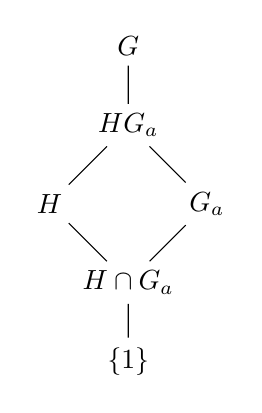
\begin{tikzpicture}
				\node (G) at (0, 0) {$G$};
				\node (HGa) at (0, -1) {$HG_a$};
				\node (H) at (-1, -2) {$H$};
				\node (Ga) at (1, -2) {$G_a$};
				\node (HcapGa) at (0, -3) {$H \cap G_a$};
				\node (1) at (0, -4) {$\{1\}$};

				\draw (1) -- (HcapGa) -- (H) -- (HGa) -- (G);
				\draw (HcapGa) -- (Ga) -- (HGa);
			\end{tikzpicture}
		\end{center}
	\end{solalph}
	\item Let $H$ and $K$ be subgroups of the group $G$. For each $x \in G$ define the $HK$ \textit{double coset} of $x$ in $G$ to be the set $HxK = \{hxk \mid h \in H, k \in K\}$.
	\begin{problems}
		\item Prove that $HxK$ is the union of the left cosets $x_1K, \ldots, x_nK$ where $\{x_1K, \ldots, x_nK\}$ is the orbit containing $xK$ of $H$ acting by left multiplication on the set of left cosets of $K$.
		\item Prove that $HxK$ is a union of right cosets of $H$.
		\item Show that $HxK$ and $HyK$ are either the same set or are disjoint for all $x, y \in G$. Show that the set of $HK$ double cosets partitions $G$.
		\item Prove that $|HxK| = |K| \cdot |H : H \cap xKx^{-1}|$.
		\item Prove that $|HxK| = |H| \cdot |K : K \cap x^{-1}Hx|$.
	\end{problems}
	\begin{solalph}
		\item Let $\oo$ be the orbit containing $xK$ of $H$ acting by left multiplication on the set of left cosets of $K$. Then $\oo = \set{hxK \mid h \in H}$, and let $\{x_1K, \ldots, x_nK\}$ be the distinct left cosets in $\oo$. Let $\kk$ be the union of these left cosets, i.e., $\kk = \bigcup_1^n x_iK$.
		
		Now pick $y \in HxK$. Then there exist $h \in H$ and $k \in K$ such that $y = hxk$. Note that $hxK \in \oo$, so there exists some $i$ such that $hxK = x_iK$. Therefore, $y = hxk \in x_iK \subseteq \kk$, hence $HxK \subseteq \kk$. If $z \in \kk$, then there exists some $i$ and some $k' \in K$ such that $z = x_ik'$. Since $x_iK \in \oo$, then there exists some $h' \in H$ such that $x_iK = h'xK$, hence $x_i = h'xk''$ for some $k'' \in K$. Therefore, $z = x_ik' = h'xkk'' \in HxK$, so $\kk \subseteq HxK$. We have shown that $HxK = \kk$, i.e., $HxK$ is the union of the left cosets $x_1K, \ldots, x_nK$.
		\item The proof is similar to that of part (a). 
		\item Let $x, y \in G$. Suppose $HxK \cap HyK \neq \varnothing$. Then there exist $h_1, h_2 \in H$ and $k_1, k_2 \in K$ such that $h_1 x k_1 = h_2 y k_2$. Rearranging, we have $y = h_2\inv h_1 x k_1 k_2\inv$, hence $y \in HxK$. Therefore, $HyK \subseteq HxK$. By symmetry, we also have $HxK \subseteq HyK$, so $HxK = HyK$. We have shown that $HxK$ and $HyK$ are either the same set or are disjoint for all $x, y \in G$. Since every element of $G$ is in some double coset of the form $HxK$, then the set of $HK$ double cosets partitions $G$.
		\item Recall that the orbit of $xK$ under this action is $\oo = \set{hxK \mid h \in H}$. By Proposition 4.2, we have $|\oo| = |H : H_{xK}|$, where $H_{xK}$ is the stabilizer of $xK$ in $H$. Observe that $H_{xK} = \set{h \in H \mid hxK = xK}$. Then $hxK = xK$ implies that there exists some $k \in K$ such that $hxk = x$, or equivalently, $h = x k x\inv$. Therefore, $H_{xK} = H \cap x K x\inv$. By part (a), we have $|HxK| = |\oo| \cdot |K| = |H : H \cap x K x\inv| \cdot |K|$.
		\item Similar to part (d).
	\end{solalph}
\end{problems}

\newpage

\subsection{Groups Acting on Themselves by Left Mutliplication---Cayley's Theorem}

\begin{problems}
	\item \label{ex4.2.1} Let $G$ be $\{1,a,b,c\}$, the Klein 4-group whose group table is written out in Section 2.5.
	\begin{problems}
		\item Label $1,a,b,c$ with the integers $1,2,4,3$, respectively, and prove that under the left regular representation of $G$ into $S_4$ the nonidentity elements are mapped as follows:
		\[a \mapsto (1\ 2)(3\ 4), \quad b \mapsto (1\ 4)(2\ 3), \quad c \mapsto (1\ 3)(2\ 4).\]
		\item Relabel $1,a,b,c$ as $1,4,2,3$, respectively, and compute the image of each element of $G$ under the left regular representation of $G$ into $S_4$. Show that the image of $G$ in $S_4$ under this labelling is the same \emph{subgroup} as the image of $G$ in part (a) (even though the nonidentity elements individually map to different permutations under the two different labellings).
	\end{problems}
	\begin{solalph}
		\item We have $a \cdot 1 = a$ so that $\sigma_a(1) = 2$. Similarly, $\sigma_a(2) = 1$. We also have $a \cdot b = c$ so that $\sigma_a(4) = 3$, and $\sigma_a(3) = 4$, and we have $a \mapsto (1\ 2)(3\ 4)$. The others are computed similarly. 
		\item Again, we have $a \cdot 1 = a$ so that $\sigma_a(1) = 4$. Similarly, $\sigma_a(4) = 1$. We also have $a \cdot b = c$ so that $\sigma_a(2) = 3$, and $\sigma_a(3) = 2$, and we have $a \mapsto (1\ 4)(2\ 3)$. For $b$, we have $b \mapsto (1\ 2)(3\ 4)$, and for $c$, we have $c \mapsto (1\ 3)(2\ 4)$. The image of $G$ in $S_4$ under this labelling is $\{1, (1\ 4)(2\ 3), (1\ 2)(3\ 4), (1\ 3)(2\ 4)\}$, which is the same subgroup as in part (a).
	\end{solalph}
	\item List the elements of $S_3$ as $1, (1\ 2), (2\ 3), (1\ 3), (1\ 2\ 3), (1\ 3\ 2)$ and label these with the integers $1,2,3,4,5,6$ respectively. Exhibit the image of each element of $S_3$ under the left regular representation of $S_3$ into $S_6$.
	\begin{sol}
		Consider $(1\ 2)$. Then we have the following computations:
		\begin{align*}
			(1\ 2) \cdot 1 & = (1\ 2) && \sigma_{(1\ 2)}(1) = 2 \\
			(1\ 2) \cdot (1\ 2) & = 1 && \sigma_{(1\ 2)}(2) = 1 \\
			(1\ 2) \cdot (2\ 3) & = (1\ 3\ 2) && \sigma_{(1\ 2)}(4) = 5 \\
			(1\ 2) \cdot (1\ 3) & = (1\ 2\ 3) && \sigma_{(1\ 2)}(3) = 6 \\
			(1\ 2) \cdot (1\ 2\ 3) & = (2\ 3) && \sigma_{(1\ 2)}(5) = 3 \\
			(1\ 2) \cdot (1\ 3\ 2) & = (1\ 3) && \sigma_{(1\ 2)}(6) = 4
		\end{align*}
		Thus, we have $(1\ 2) \mapsto (1\ 2)(3\ 6\ 4\ 5)$. We calculate that $(2\ 3) \mapsto (1\ 3\ 5\ 2)(4\ 6)$. Since $(1\ 2)(2\ 3) = (1\ 2\ 3)$, then
		\[(1\ 2\ 3) \mapsto (1\ 2)(3\ 6\ 4\ 5)(1\ 3\ 5\ 2)(4\ 6) = (1\ 5\ 6)(2\ 4\ 3)\]
		Continuing in this way, we find that the images of the elements of $S_3$ under the left regular representation are as follows:
		\begin{align*}
			1 & \mapsto 1 \\
			(1\ 2) & \mapsto (1\ 2)(3\ 6\ 4\ 5) \\
			(2\ 3) & \mapsto (1\ 3\ 5\ 2)(4\ 6) \\
			(1\ 3) & \mapsto (1\ 4)(2\ 6)(3\ 5) \\
			(1\ 2\ 3) & \mapsto (1\ 5\ 6)(2\ 4\ 3) \\
			(1\ 3\ 2) & \mapsto (1\ 6\ 5)(2\ 3\ 4) \qh
		\end{align*}
	\end{sol}
	\item \label{ex4.2.3} Let $r$ and $s$ be the usual generators for the dihedral group of order 8.
	\begin{problems}
		\item List the elements of $D_8$ as $1, r, r^2, r^3, s, sr, sr^2, sr^3$ and label these with the integers $1,2,\dots,8$ respectively. Exhibit the image of each element of $D_8$ under the left regular representation of $D_8$ into $S_8$.
		\item Relabel this same list of elements of $D_8$ with the integers $1,3,5,7,2,4,6,8$ respectively and recompute the image of each element of $D_8$ under the left regular representation with respect to this new labelling. Show that the two subgroups of $S_8$ obtained in parts (a) and (b) are different.
	\end{problems}
	\begin{solalph}
		\item We calculate $\sigma_r = (1\ 2\ 3\ 4)(5\ 8\ 7\ 6)$ and $\sigma_s = (1\ 5)(2\ 6)(3\ 7)(4\ 8)$. Continuing in this way, we find that the images of the elements of $D_8$ under the left regular representation are as follows:
		\begin{align*}
			1 & \mapsto 1 & s & \mapsto (1\ 5)(2\ 6)(3\ 7)(4\ 8) \\
			r & \mapsto (1\ 2\ 3\ 4)(5\ 8\ 7\ 6) & sr & \mapsto (1\ 6)(2\ 7)(3\ 8)(4\ 5) \\
			r^2 & \mapsto (1\ 3)(2\ 4)(5\ 7)(6\ 8) & sr^2 & \mapsto (1\ 7)(2\ 8)(3\ 5)(4\ 6) \\
			r^3 & \mapsto (1\ 4\ 3\ 2)(5\ 6\ 7\ 8) & sr^3 & \mapsto (1\ 8)(2\ 5)(3\ 6)(4\ 7)
		\end{align*}
		\item The images of $D_8$ under the left regular representation with respect to this new labelling are as follows:
		\begin{align*}
			1 & \mapsto 1 & s & \mapsto (1\ 2)(3\ 4)(5\ 6)(7\ 8) \\
			r & \mapsto (1\ 3\ 5\ 7)(2\ 8\ 6\ 4) & sr & \mapsto (1\ 4)(2\ 7)(3\ 6)(5\ 8) \\
			r^2 & \mapsto (1\ 5)(3\ 7)(2\ 6)(4\ 8) & sr^2 & \mapsto (1\ 6)(2\ 5)(3\ 8)(4\ 7) \\
			r^3 & \mapsto (1\ 7\ 5\ 3)(2\ 4\ 6\ 8) & sr^3 & \mapsto (1\ 8)(2\ 3)(4\ 5)(6\ 7)
		\end{align*}
		Clearly, the two subgroups of $S_8$ obtained in parts (a) and (b) are different since, for example, the image of $r$ in part (a) is a product of two 4-cycles while the image of $r$ in part (b) is a product of two 4-cycles but with different elements.
	\end{solalph}
	\item \label{ex4.2.4} Use the left regular representation of $Q_8$ to produce two elements of $S_8$ which generate a subgroup of $S_8$ isomorphic to the quaternion group $Q_8$.
	\begin{sol}
		At minimum, we have that $Q_8 = \gen{i, j}$ (any 2 elements of order 4 can be used), so we compute the images of $i$ and $j$ under the left regular representation. We label $Q_8$ as $1, -1, i, -i, j, -j, k, -k$ and label these with the integers $1,2 \ldots 8$ respectively. We find that
		\begin{align*}
			i & \mapsto \sigma_i = (1\ 3\ 4\ 2)(5\ 7)(6\ 8) \\
			j & \mapsto \sigma_j = (1\ 5\ 2\ 6)(3\ 8)(4\ 7)
		\end{align*}
		Hence $Q_8 \cong \gen{\sigma_i, \sigma_j} \leq S_8$.
	\end{sol}
	\item \label{ex4.2.5} Let $r$ and $s$ be the usual generators for the dihedral group of order 8 and let $H = \langle s \rangle$. List the left cosets of $H$ in $D_8$ as $1H, rH, r^2H$ and $r^3H$.
	\begin{problems}
		\item Label these cosets with the integers $1,2,3,4$, respectively. Exhibit the image of each element of $D_8$ under the representation $\pi_H$ of $D_8$ into $S_4$ obtained from the action of $D_8$ by left multiplication on the set of 4 left cosets of $H$ in $D_8$. Deduce that this representation is faithful (i.e., the elements of $S_4$ obtained form a subgroup isomorphic to $D_8$).
		\item Repeat part (a) with the list of cosets relabelled by the integers $1,3,2,4$, respectively. Show that the permutations obtained from this labelling form a subgroup of $S_4$ that is different from the subgroup obtained in part (a).
		\item Let $K = \langle sr \rangle$, list the cosets of $K$ in $D_8$ as $1K, rK, r^2K$ and $r^3K$, and label these with the integers $1,2,3,4$. Prove that, with respect to this labelling, the image of $D_8$ under the representation $\pi_K$ obtained from left multiplication on the cosets of $K$ is the same \emph{subgroup} of $S_4$ as in part (a) (even though the subgroups $H$ and $K$ are different and some of the elements of $D_8$ map to different permutations under the two homomorphisms).
	\end{problems}
	\begin{solalph}
		\item We have $\pi_H(r) = (1\ 2\ 3\ 4)$ and $\pi_H(s) = (2\ 4)$. We continue in this way to find that the images of the elements of $D_8$ under $\pi_H$ are:
		\begin{align*}
			\pi_H(1) & = 1 & \pi_H(s) & = (2\ 4) \\
			\pi_H(r) & = (1\ 2\ 3\ 4) & \pi_H(sr) & = (1\ 2)(3\ 4) \\
			\pi_H(r^2) & = (1\ 3)(2\ 4) & \pi_H(sr^2) & = (1\ 3) \\
			\pi_H(r^3) & = (1\ 4\ 3\ 2) & \pi_H(sr^3) & = (1\ 4)(2\ 3)
		\end{align*}
		so that the subgroup $\gen{\pi_H(r), \pi_H(s)} \leq S_4$ is isomorphic to $D_8$. Since the kernel of $\pi_H$ is trivial, then the representation is faithful.
		\item The new labelling affords the permutations $\pi_H(r) = (1\ 3\ 2\ 4)$ and $\pi_H(s) = (3\ 4)$. We have the following images:
		\begin{align*}
			\pi_H(1) & = 1 & \pi_H(s) & = (3\ 4) \\
			\pi_H(r) & = (1\ 3\ 2\ 4) & \pi_H(sr) & = (1\ 3)(2\ 4) \\
			\pi_H(r^2) & = (1\ 2)(3\ 4) & \pi_H(sr^2) & = (1\ 2) \\
			\pi_H(r^3) & = (1\ 4\ 2\ 3) & \pi_H(sr^3) & = (1\ 4)(2\ 3)
		\end{align*}
		Moreover, the subgroup is different from that in part (a) since, for example, the image of $r$ in part (a) is $(1\ 2\ 3\ 4)$ while the image of $r$ in this part is $(1\ 3\ 2\ 4)$.
		\item Under $\pi_K$, we have $\pi_K(r) = (1\ 2\ 3\ 4)$ and $\pi_K(s) = (1\ 2)(3\ 4)$. With respect to this labeling, we have the subgroup $\wh K = \gen{(1\ 2\ 3\ 4), (1\ 2)(3\ 4)}$. Let $\wh H$ be the subgroup obtained in part (a). Note that $(1\ 2\ 3\ 4)$ is contained in both $\wh H$ and $\wh K$. Moreover, we have following:
		\[(1\ 2\ 3\ 4)(2\ 4)(1\ 4\ 3\ 2) = (1\ 2)(3\ 4) \in \wh H \longand (1\ 2\ 3\ 4)^2(1\ 2)(3\ 4) = (2\ 4) \in \wh K\]
		so that both subgroups contain the other generator of the other subgroup. Therefore, $\wh H = \wh K$.
	\end{solalph}
    \item Let $r$ and $s$ be the usual generators for the dihedral group of order 8 and let $N = \langle r^2 \rangle$. List the left cosets of $N$ in $D_8$ as $1N, rN, sN$ and $srN$. Label these cosets with the integers $1,2,3,4$ respectively. Exhibit the image of each element of $D_8$ under the representation $\pi_N$ of $D_8$ into $S_4$ obtained from the action of $D_8$ by left multiplication on the set of 4 left cosets of $N$ in $D_8$. Deduce that this representation is not faithful and prove that $\pi_N(D_8)$ is isomorphic to the Klein 4-group.
	\begin{sol}
		We have $\pi_N(r) = (1\ 2)(3\ 4)$ and $\pi_N(s) = (1\ 3)(2\ 4)$. Continuing in this way, we find that the images of the elements of $D_8$ under $\pi_N$ are:
		\begin{align*}
			\pi_N(1) & = 1 & \pi_N(s) & = (1\ 3)(2\ 4) \\
			\pi_N(r) & = (1\ 2)(3\ 4) & \pi_N(sr) & = (1\ 4)(2\ 3) \\
			\pi_N(r^2) & = 1 & \pi_N(sr^2) & = (1\ 3)(2\ 4) \\
			\pi_N(r^3) & = (1\ 2)(3\ 4) & \pi_N(sr^3) & = (1\ 4)(2\ 3)
		\end{align*}
		Since $\ker(\pi_N)$ contains the nontrivial element $r^2$, then the representation is not faithful. Moreover, we have $\pi_N(D_8) = \{1, (1\ 2)(3\ 4), (1\ 3)(2\ 4), (1\ 4)(2\ 3)\}$, which is isomorphic to the Klein 4-group.
	\end{sol}
    \item Let $Q_8$ be the quaternion group of order 8.
	\begin{problems}
		\item Prove that $Q_8$ is isomorphic to a subgroup of $S_8$.
		\item Prove that $Q_8$ is not isomorphic to a subgroup of $S_n$ for any $n \le 7$. [If $Q_8$ acts on any set $A$ of order $\le 7$ show that the stabilizer of any point $a \in A$ must contain the subgroup $\langle -1 \rangle$.]
	\end{problems}
	\begin{solalph}
		\item This is done in \hyperref[ex4.2.4]{Exercise 4.2.4}.
		\item Let $Q_8$ act on a set $A$ of order $n \leq 7$. For any $a \in A$, consider the orbit $\oo_a$ of $a$ under this action. By Proposition 4.2, we have $|\oo_a| = |Q_8 : (Q_8)_a|$, where $(Q_8)_a$ is the stabilizer of $a$ in $Q_8$. Since $|\oo_a|$ divides $|A| \leq 7$, then $|\oo_a|$ must be 1, 2, 4, or 7. However, since $Q_8$ has no subgroup of index 7, then $|\oo_a|$ cannot be 7. If $|\oo_a| = 4$, then $(Q_8)_a$ has order 2, but the only subgroup of order 2 in $Q_8$ is $\langle -1 \rangle$. If $|\oo_a| = 2$, then $(Q_8)_a$ has order 4, and the only subgroups of order 4 in $Q_8$ are $\langle i \rangle$, $\langle j \rangle$, and $\langle k \rangle$, all of which contain $\langle -1 \rangle$. If $|\oo_a| = 1$, then $(Q_8)_a = Q_8$, which also contains $\langle -1 \rangle$. Therefore, in all cases, the stabilizer $(Q_8)_a$ contains $\langle -1 \rangle$. Since this holds for all $a \in A$, then $\langle -1 \rangle$ is contained in the kernel of the action. The action is not faithful, hence $Q_8$ cannot be isomorphic to a subgroup of $S_n$ for any $n \leq 7$.
	\end{solalph}
    \item Prove that if $H$ has finite index $n$ then there is a normal subgroup $K$ of $G$ with $K \le H$ and $|G : K| \le n!$.
	\begin{sol}
		Let $G$ act by left multiplication on the set of left cosets of $H$ in $G$. Then we have the homomorphism $\phi : G \to S_n$, which is the permutation representation of $G$ on $G/H$. Let $K = \ker(\phi) \subseteq H$, since $g \in K$ if and only if $gH = H$. By the First Isomorphism Theorem, we have $G/K \cong \phi(G) \leq S_n$, so that $|G : K| = |G/K| = |\phi(G)|$ divides $n!$. Therefore, $|G : K| \leq n!$.
	\end{sol}
    \item Prove that if $p$ is a prime and $G$ is a group of order $p^\alpha$ for some $\alpha \in \mathbb{Z}^+$, then every subgroup of index $p$ is normal in $G$. Deduce that every group of order $p^2$ has a normal subgroup of order $p$.
	\begin{sol}
		Let $H$ be a subgroup of $G$ with index $p$. Then $|G : H| = p$, so the action of $G$ on the left cosets of $H$ in $G$ gives a homomorphism $\phi : G \to S_p$. Since $|G| = p^\alpha$, then by Lagrange's Theorem, the order of $\phi(G)$ divides $p^\alpha$. However, the only subgroups of $S_p$ whose order divides $p^\alpha$ are the trivial group and groups of order $p$. Since $\phi(G)$ acts transitively on the $p$ cosets of $H$, then $\phi(G)$ cannot be trivial. Therefore, $|\phi(G)| = p$, which is prime, so $\phi(G)$ is cyclic and hence abelian. The kernel of $\phi$ is a normal subgroup of $G$ contained in $H$. Since the image $\phi(G)$ has order $p$, then by the First Isomorphism Theorem, we have $|G : \ker(\phi)| = p$. But since $\ker(\phi) \subseteq H$ and both have index $p$, then $\ker(\phi) = H$. Therefore, $H$ is normal in $G$.

		To deduce that every group of order $p^2$ has a normal subgroup of order $p$, let $G$ be a group of order $p^2$. By Cauchy's Theorem, there exists an element of order $p$ in $G$, which generates a subgroup $H$ of order $p$. Since the index of $H$ in $G$ is $p$, by the previous result, $H$ is normal in $G$.
	\end{sol}
    \item Prove that every non-abelian group of order 6 has a nonnormal subgroup of order 2. Use this to classify groups of order 6. [Produce an injective homomorphism into $S_3$.]
	\begin{sol}
		Note that $2 \mid 6$ and $3 \mid 6$. By Cauchy's Theorem, there exists subgroups $H$ and $K$ of orders 2 and 3 respectively. Let $H = \set{1, h}$, suppose it is normal, and let $g \in G - H$. Since $H \nsub G$, then $gHg\inv = H$. In particular, $ghg\inv \in H$, so either $ghg\inv = 1$ or $ghg\inv = h$. Since the first case implies $h = 1$, it must be that $ghg\inv = h$, or $gh = hg$. Then $h$ commutes with every element. Moreover, we may use \hyperref[ex3.3.3]{Exercise 3.3.3} to conclude that $G = HK$ since $H \nsub G$. Since $K$ is also abelian as it is cyclic, then $G = hk$ for $h \in H$ and $k \in K$, implying that $G$ is abelian, a contradiction. Therefore, $H$ is not normal in $G$.

		To classify groups of order 6, let $G$ be a group of order 6. If $G$ is abelian, then $G \cong \z_6 \cong \z_2 \times \z_3$. If $G$ is non-abelian, then by the above result, $G$ has a nonnormal subgroup $H$ of order 2. Let $K$ be the subgroup of order 3. Then $G = HK$. Let $G$ act by left multiplication on the left cosets of $K$ in $G$. This action gives a homomorphism $\phi : G \to S_3$. Since $H$ is not normal in $G$, then the action is nontrivial, so $\phi$ is injective. Therefore, $G \cong \phi(G) \leq S_3$. Since $|G| = 6 = |S_3|$, then $\phi(G) = S_3$, and hence $G \cong S_3$.
	\end{sol}
    \item \label{ex4.2.11} Let $G$ be a finite group and let $\pi : G \to S_G$ be the left regular representation. Prove that if $x$ is an element of $G$ of order $n$ and $|G| = mn$, then $\pi(x)$ is a product of $m$ $n$-cycles. Deduce that $\pi(x)$ is an odd permutation if and only if $|x|$ is even and $\abs G/\abs x$ is odd.
	\begin{sol}
		Let $x \in G$ with $\abs x = n$. Consider the action of $\langle x \rangle$ on $G$ by left multiplication. The orbit of any $g \in G$ under this action is $\oo_g = \set{x^k g \mid k = 0, 1, \ldots, n-1}$. Since $\abs x = n$, then $|\oo_g| = n$ for all $g \in G$. By Proposition 4.2, we have $|\oo_g| = |\langle x \rangle : (\langle x \rangle)_g|$, where $(\langle x \rangle)_g$ is the stabilizer of $g$ in $\langle x \rangle$. Since $|\oo_g| = n$, then $(\langle x \rangle)_g$ is trivial for all $g \in G$. Therefore, the orbits of this action partition $G$ into subsets of size $n$. Since $|G| = mn$, there are exactly $m$ such orbits. Each orbit corresponds to an $n$-cycle in the permutation $\pi(x)$. Therefore, $\pi(x)$ is a product of $m$ $n$-cycles.

		To determine when $\pi(x)$ is an odd permutation, we note that an $n$-cycle is an odd permutation if and only if $n$ is even. Since $\pi(x)$ is a product of $m$ $n$-cycles, the parity of $\pi(x)$ is determined by the parity of $m$ and $n$. Specifically, $\pi(x)$ is odd if and only if $n$ is even and $m$ is odd. Thus, $\pi(x)$ is an odd permutation if and only if $|x|$ is even and $|G|/|x|$ is odd.
	\end{sol}
    \item \label{ex4.2.12} Let $G$ and $\pi$ be as in the preceding exercise. Prove that if $\pi(G)$ contains an odd permutation then $G$ has a subgroup of index 2. [Use \hyperref[ex3.3.3]{Exercise 3.3.3}.]
	\begin{sol}
		Recall the $\ep$ homomorphism from Proposition 3.23. Moreover, $\pi$ is a homomorphism from $G$ to $S_G$. Consider the composition $\ep \circ \pi : G \to \set{\pm 1}$. Since $\pi(G)$ contains an odd permutation, then $\ep \circ \pi$ is surjective. By the First Isomorphism Theorem, we have $G/\ker(\ep \circ \pi) \cong \set{\pm 1}$, so that $|\ker(\ep \circ \pi)| = |G|/2$. Therefore, $\ker(\ep \circ \pi)$ is a subgroup of $G$ of index 2.
	\end{sol}
    \item Prove that if $|G| = 2k$ where $k$ is odd then $G$ has a subgroup of index 2. [Use Cauchy's Theorem to produce an element of order 2 and then use the preceding two exercises.]
	\begin{sol}
		By Cauchy's Theorem, there exists $x \in G$ such that $\abs x = 2$. Then $\pi(x)$ is of order 2 and is hence a product of disjoint transpositions. Since $|G| = 2k$ with $k$ odd, then use $m = k$ and $n = 2$ in \hyperref[ex4.2.11]{Exercise 4.2.11} along with even $\abs x$ to conclude that $\pi(x)$ is an odd permutation. By the \hyperref[ex4.2.12]{Exercise 4.2.12}, $G$ has a subgroup of index 2.
	\end{sol}
    \item Let $G$ be a finite group of composite order $n$ with the property that $G$ has a subgroup of order $k$ for each positive integer $k$ dividing $n$. Prove that $G$ is not simple.
    \begin{sol}
		Let $S$ be the set of all prime factors of $n$. By the Well Ordering Principle, this has a minimal element $p$. By hypothesis, $G$ has a subgroup $P$ of order $n/p$ with index $p$. By Corollary 4.5, $P$ is normal in $G$ since $p$ is the smallest prime dividing $n$. Therefore, $G$ is not simple.
	\end{sol}
\end{problems}

\newpage

\subsection{Groups Acting on Themselves by Conjugation---The Class Equation}

Let $G$ be a group.

\begin{problems}
	\item  Suppose $G$ has a left action on a set $A$, denoted by $g \cdot a$ for all $g \in G$ and $a \in A$. Denote the corresponding right action on $A$ by $a \cdot g$. Prove that the (equivalence) relations $\sim$ and $\sim'$ defined by
	\[ a \sim b \quad \text{if and only if} \quad a = g \cdot b \quad \text{ for some } g \in G \]
	and
	\[ a \sim' b \quad \text{if and only if} \quad a = b \cdot g \quad \text{ for some } g \in G \]
	are the same relation (i.e., $a \sim b$ if and only if $a \sim' b$).
	\begin{sol}
		If $a \sim b$, there exists $g \in G$ such that $a = g \cdot b$. Let $h = g\inv$. Then $b = h \cdot a$, so $a = b \cdot g$. Thus, $a \sim' b$. Conversely, if $a \sim' b$, there exists $g \in G$ such that $a = b \cdot g$. Let $h = g\inv$. Then $b = h \cdot a$, so $a = g \cdot b$. Thus, $a \sim b$. Therefore, the relations $\sim$ and $\sim'$ are the same.
	\end{sol}
	\item \label{ex4.3.2} Find all conjugacy classes and their sizes in the following groups:
	\begin{problems}
		\item $D_8$
		\item $Q_8$
		\item $A_4$
	\end{problems}
	\begin{solalph}
		\item Discussed in the text, the conjugacy classes of $D_8$ are $\{1\}$, $\{r^2\}$, $\{r, r^3\}$, $\{s, sr^2\}$, and $\{sr, sr^3\}$ with sizes 1, 1, 2, 2, and 2 respectively.
		\item Again discussed in the text, the conjugacy classes of $Q_8$ are $\{1\}$, $\{-1\}$, $\{i, -i\}$, $\{j, -j\}$, and $\{k, -k\}$ with sizes 1, 1, 2, 2, and 2 respectively.
		\item We proceed similarly as the text. The possible cycle types are $1, (1\ 2\ 3)$, and $(1\ 2)(3\ 4)$.
		
		For $(1\ 2\ 3)$, we have $C_{A_4}((1\ 2\ 3)) = \gen{(1\ 2\ 3)}$ since the only permutation that fixes 1, 2, and 3 is the identity. Therefore, the conjugacy class of $(1\ 2\ 3)$ has size $12/3 = 4$. However, there are 8 3-cycles in $A_4$, so there exists a 3-cycle $\sigma \in A_4$ not in the conjugacy class of $(1\ 2\ 3)$. By similar reasoning, the conjugacy class of $\sigma$ also has size 4. There are then 2 conjugacy classes of size 4 corresponding to the 3-cycles.

		For $(1\ 2)(3\ 4)$, it is trivial to calculate that the remaining double transpositions are in its conjugacy class. Therefore, the conjugacy class of $(1\ 2)(3\ 4)$ has size 3.
	\end{solalph}
	\item Find all conjugacy classes and their sizes in the following groups:
	\begin{problems}
		\item $Z_2 \times S_3$
		\item $S_3 \times S_3$
		\item $Z_3 \times A_4$
	\end{problems}
	\begin{sol}
		We first prove a (somewhat) trivial idea: if $G$ and $H$ are groups, let $g \in G$ and $h \in H$. Let $\kk_g$ and $\kk_h$ be the conjugacy classes of $g$ in $G$ and $h$ in $H$ respectively. Then $\kk_{(g,h)} = \kk_g \times \kk_h$ is the conjugacy class of $(g,h)$ in $G \times H$. To see this, note that for any $(x,y) \in G \times H$, we have
		\[(x,y)(g,h)(x,y)\inv = (xgx\inv, yhy\inv) \in \kk_g \times \kk_h.\]
		Conversely, for any $(g', h') \in \kk_g \times \kk_h$, there exist $x \in G$ and $y \in H$ such that $g' = xgx\inv$ and $h' = yhy\inv$. Therefore, $(g', h') = (x,y)(g,h)(x,y)\inv$, so $(g', h')$ is in the conjugacy class of $(g,h)$ in $G \times H$. This result shows two important things: the conjugacy classes of $G \times H$ are precisely the products of the conjugacy classes of $G$ and $H$, and the size of the conjugacy class of $(g,h)$ in $G \times H$ is the product of the sizes of the conjugacy classes of $g$ in $G$ and $h$ in $H$. We now use this to answer the question.
		\begin{problems}
			\item Let $Z_2 = \gen x$. The conjugacy classes $\kk_1$ and $\kk_x$ of $Z_2$ have sizes 1 and 1 respectively. For $S_3$, the partitions of 3 are 3 1-cycles, 2-cycle and 1-cycle, and a 3-cycle with representatives $1$, $(1\ 2)$, and $(1\ 2\ 3)$ respectively. Since $C_{S_3}((1\ 2)) = \gen{(1\ 2)}$ and $C_{S_3}((1\ 2\ 3)) = \gen{(1\ 2\ 3)}$, then the conjugacy classes $\kk_1$, $\kk_{(1\ 2)}$, and $\kk_{(1\ 2\ 3)}$ of $S_3$ have sizes 1, 3, and 2 respectively. Therefore, $Z_2 \times S_3$ has 6 conjugacy classes of size 1, 3, 2, 1, 3, and 2 respectively.
			\item By the above, $S_3$ has 3 conjugacy classes of sizes 1, 3, and 2 respectively. Then $S_3 \times S_3$ has 9 conjugacy classes with sizes $1, 3, 2, 3, 9, 6, 2, 6,$ and $4$ respectively.
			\item $Z_3$ has 3 conjugacy classes of size 1 each. From \hyperref[ex4.3.2]{Exercise 4.3.2}, we know that $A_4$ has 4 conjugacy classes of sizes 1, 4, 4, and 3. Therefore, $Z_3 \times A_4$ has 12 conjugacy classes with sizes $1, 4, 4, 3, 1, 4, 4, 3, 1, 4, 4,$ and $3$ respectively. \qh
		\end{problems}
	\end{sol}
	\item Prove that if $S \subseteq G$ and $g \in G$ then $gN_G(S)g^{-1} = N_G(gSg^{-1})$ and $gC_G(S)g^{-1} = C_G(gSg^{-1}).$
	\begin{sol}
		Suppose $x \in gN_G(S)g\inv$, and consider $xgSg\inv x\inv$. Since $x = gng\inv$ for some $n \in N_G(S)$, then we have $gng\inv gSg\inv gn\inv g\inv = g n S n\inv g\inv = g S g\inv$, so that $x \in N_G(gSg\inv)$. Conversely, suppose $x \in N_G(gSg\inv)$. Then $xgSg\inv x\inv = gSg\inv$. Letting $n = g\inv x g$, we have $n S n\inv = S$, so $n \in N_G(S)$ and hence $x \in gN_G(S)g\inv$. Therefore, $gN_G(S)g\inv = N_G(gSg\inv)$.

		Suppose $x \in gC_G(S)g\inv$, and consider $xsx\inv$ for some $s \in gSg\inv$. Since $x = gng\inv$ for some $n \in C_G(S)$, then we have $gng\inv s g n\inv g\inv = g n (g\inv s g) n\inv g\inv = g (g\inv s g) g\inv = s$, so that $x \in C_G(gSg\inv)$. Conversely, suppose $x \in C_G(gSg\inv)$. Then $xsx\inv = s$ for all $s \in gSg\inv$. Letting $n = g\inv x g$, we have $n t n\inv = t$ for all $t \in S$, so $n \in C_G(S)$ and hence $x \in gC_G(S)g\inv$. Therefore, $gC_G(S)g\inv = C_G(gSg\inv)$.
	\end{sol}
	\item If the center of $G$ is of index $n$, prove that every conjugacy class has at most $n$ elements.
	\begin{sol}
		Let $\kk_g$ be the conjugacy class of some $g \in G$. By Proposition 4.6, we have $|\kk_g| = |G : C_G(g)|$. Since $Z(G) \leq C_G(g)$ for all $g \in G$, Lagrange's Theorem shows that $|Z(G)|$ divides $|C_G(g)|$. Therefore, $|G : C_G(g)|$ divides $|G : Z(G)| = n$. Hence, $|\kk_g| \leq n$.
	\end{sol}
	\item Assume $G$ is a non-abelian group of order $15$. Prove that $Z(G)=1$. Use the fact that $\langle g \rangle \le C_G(g)$ for all $g \in G$ to show that there is at most one possible class equation for $G$. [Use \hyperref[ex3.1.36]{Exercise 3.1.36}.]
	\begin{sol}
		Recall that $Z(G) \leq G$. Since $G$ is non-abelian, then $Z(G) \neq G$. Assume $1 < Z(G) < 15$. By Lagrange's Theorem, $Z(G)$ has order 3 or 5. If $|Z(G)| = 3$, then $|G/Z(G)| = 5$ and $G/Z(G) \cong Z_5$. If $|Z(G)| = 5$, then $|G/Z(G)| = 3$ and $G/Z(G) \cong Z_3$. In either case, $G/Z(G)$ is cyclic by Corollary 3.10, and \hyperref[ex3.1.36]{Exercise 3.1.36} implies that $G$ is abelian, a contradiction. Therefore, $Z(G) = 1$.

		Now suppose $g \in G$ is nonidentity. Since $\langle g \rangle \leq C_G(g)$, then $|C_G(g)|$ is 3, 5, or 15 by Lagrange's Theorem. If $|C_G(g)| = 15$, then $C_G(g) = G$, so $g \in Z(G)$, a contradiction. Therefore, $|C_G(g)|$ is 3 or 5 for all nonidentity $g \in G$. By Proposition 4.6, we have $|\kk_g| = |G : C_G(g)|$, so that $|\kk_g|$ is 5 or 3 respectively. The identity element forms a conjugacy class of size 1, and the class equation must involve a summation of sizes 3 and 5 that adds to 14. The only such combination is three classes of size 3 and one class of size 5. Therefore, the class equation of $G$ is $15 = 1 + 3 + 3 + 3 + 5$.
	\end{sol}
	\item For $n=3,4,6,$ and $7$ make lists of the partitions of $n$ and give representatives for the corresponding conjugacy classes of $S_n$.
	\begin{sol}
		$n = 3$:
		\[\begin{array}{c|c}
			\textbf{Partition of 3} & \textbf{Representative of Cycle Type} \\
			\hline
			1, 1, 1 & 1 \\
			2, 1 & (1\ 2) \\
			3 & (1\ 2\ 3)
		\end{array}\]
		$n = 4$:
		\[\begin{array}{c|c}
			\textbf{Partition of 4} & \textbf{Representative of Cycle Type} \\
			\hline
			1, 1, 1, 1 & 1 \\
			2, 1, 1 & (1\ 2) \\
			2, 2 & (1\ 2)(3\ 4) \\
			3, 1 & (1\ 2\ 3) \\
			4 & (1\ 2\ 3\ 4)
		\end{array}\]
		$n = 6$:
		\[\begin{array}{c|c}
			\textbf{Partition of 6} & \textbf{Representative of Cycle Type} \\
			\hline
			1, 1, 1, 1, 1, 1 & 1 \\
			2, 1, 1, 1, 1 & (1\ 2) \\
			2, 2, 1, 1 & (1\ 2)(3\ 4) \\
			2, 2, 2 & (1\ 2)(3\ 4)(5\ 6) \\
			3, 1, 1, 1 & (1\ 2\ 3) \\
			3, 2, 1 & (1\ 2\ 3)(4\ 5) \\
			3, 3 & (1\ 2\ 3)(4\ 5\ 6) \\
			4, 1, 1 & (1\ 2\ 3\ 4) \\
			4, 2 & (1\ 2\ 3\ 4)(5\ 6) \\
			5, 1 & (1\ 2\ 3\ 4\ 5) \\
			6 & (1\ 2\ 3\ 4\ 5\ 6)
		\end{array}\]
		$n = 7$:
		\[\begin{array}{c|c}
			\textbf{Partition of 7} & \textbf{Representative of Cycle Type} \\
			\hline
			1, 1, 1, 1, 1, 1, 1 & 1 \\
			2, 1, 1, 1, 1, 1 & (1\ 2) \\
			2, 2, 1, 1, 1 & (1\ 2)(3\ 4) \\
			2, 2, 2, 1 & (1\ 2)(3\ 4)(5\ 6) \\
			3, 1, 1, 1, 1 & (1\ 2\ 3) \\
			3, 2, 1, 1 & (1\ 2\ 3)(4\ 5) \\
			3, 2, 2 & (1\ 2\ 3)(4\ 5)(6\ 7) \\
			3, 3, 1 & (1\ 2\ 3)(4\ 5\ 6) \\
			4, 1, 1, 1 & (1\ 2\ 3\ 4) \\
			4, 2, 1 & (1\ 2\ 3\ 4)(5\ 6) \\
			4, 3 & (1\ 2\ 3\ 4)(5\ 6\ 7) \\
			5, 1, 1 & (1\ 2\ 3\ 4\ 5) \\
			5, 2 & (1\ 2\ 3\ 4\ 5)(6\ 7) \\
			6, 1 & (1\ 2\ 3\ 4\ 5\ 6) \\
			7 & (1\ 2\ 3\ 4\ 5\ 6\ 7)
		\end{array} \qh\]
	\end{sol}
	\item Prove that $Z(S_n)=1$ for all $n \ge 3$.
	\begin{sol}
		Suppose $\sigma \in Z(S_n)$ for some $n \geq 3$. Then $\sigma$ commutes with every element of $S_n$. In particular, $\sigma$ commutes with all transpositions (the set of which generate $S_n$). Let $(a\ b)$ be any transposition in $S_n$. Then we have $\sigma(a\ b)\sigma\inv = (a\ b)$. This implies that $(\sigma(a)\ \sigma(b)) = (a\ b)$, so $\sigma(a) = a$ and $\sigma(b) = b$. Since $a$ and $b$ were arbitrary, $\sigma$ fixes every element of $\{1, 2, \ldots, n\}$. Therefore, $\sigma$ is the identity permutation. Hence, $Z(S_n) = \{1\}$ for all $n \geq 3$.
	\end{sol}
	\item Show that $|C_{S_n}((1\ 2)(3\ 4))| = 8 (n-4)!$ for all $n \ge 4$. Determine the elements in this centralizer explicitly.
	\begin{sol}
		The $(n - 4)!$ factor arises from the fact that permutations on the $n - 4$ integers not involved in the cycle $(1\ 2)(3\ 4)$ commute with it. Therefore, we need only consider the permutations of $\{1, 2, 3, 4\}$ that commute with $(1\ 2)(3\ 4)$. Computing $C_{S_4}((1\ 2)(3\ 4))$ directly, the permutations that fall in this set need to leave $(1\ 2)(3\ 4)$ unchanged, or swap the two transpositions. The permutations that leave $(1\ 2)(3\ 4)$ unchanged are $1$, $(1\ 2)$, $(3\ 4)$, and $(1\ 2)(3\ 4)$. The permutations that swap the two transpositions are $(1\ 3)(2\ 4)$, $(1\ 4)(2\ 3)$, $(1\ 3\ 2\ 4)$, and $(1\ 4\ 2\ 3)$. Therefore, 
		\[C_{S_4}((1\ 2)(3\ 4)) = \{1, (1\ 2), (3\ 4), (1\ 2)(3\ 4), (1\ 3)(2\ 4), (1\ 4)(2\ 3), (1\ 3\ 2\ 4), (1\ 4\ 2\ 3)\},\]
		which has size 8. Combining this with the $(n - 4)!$ factor, we have $|C_{S_n}((1\ 2)(3\ 4))| = 8(n - 4)!$ for all $n \geq 4$.
	\end{sol}
	\item Let $\sigma$ be the 5-cycle $(1\ 2\ 3\ 4\ 5)$ in $S_5$. In each of (a) to (c) find an explicit element $\tau \in S_5$ which accomplishes the specified conjugation:
	\begin{problems}
		\item $\tau \sigma \tau^{-1} = \sigma^2$
		\item $\tau \sigma \tau^{-1} = \sigma^{-1}$
		\item $\tau \sigma \tau^{-1} = \sigma^{-2}$
	\end{problems}
	\begin{solalph}
		\item $\sigma^2 = (1\ 3\ 5\ 2\ 4)$. Then $\tau = (2\ 3\ 5\ 4)$.
		\item $\sigma^{-1} = (1\ 5\ 4\ 3\ 2)$. Then $\tau = (1\ 5)(2\ 4)$.
		\item $\sigma^{-2} = (1\ 4\ 2\ 5\ 3)$. Then $\tau = (2\ 4\ 5\ 3)$.
	\end{solalph}
	\item In each of (a) -- (d) determine whether $\sigma_1$ and $\sigma_2$ are conjugate. If they are, given an explicit permutation $\tau$ such that $\tau \sigma_1 \tau^{-1} = \sigma_2$.
	\begin{problems}
		\item $\sigma_1 = (1\ 2)(3\ 4\ 5)$ and $\sigma_2 = (1\ 2\ 3)(4\ 5)$
		\item $\sigma_1 = (1\ 5)(3\ 7\ 2)(10\ 6\ 8\ 11)$ and $\sigma_2 = (3\ 7\ 5\ 10)(4\ 9)(13\ 11\ 2)$
		\item $\sigma_1 = (1\ 5)(3\ 7\ 2)(10\ 6\ 8\ 11)$ and $\sigma_2 = \sigma_1^3$
		\item $\sigma_1 = (1\ 3)(2\ 4\ 6)$ and $\sigma_2 = (3\ 5)(2\ 4)(5\ 6)$
	\end{problems}
	\begin{solalph}
		\item Rewrite $\sigma_2$ as $(4\ 5)(1\ 2\ 3)$ so that both have the same cycle type. Then $\tau = (1\ 4\ 2\ 5\ 3)$.
		\item Rewrite $\sigma_2$ as $(4\ 9)(13\ 11\ 2)(3\ 7\ 5\ 10)$. Then $\tau = (1\ 4)(8\ 5\ 9)(6\ 7\ 11\ 10\ 3\ 13)$.
		\item Note that $\sigma_2 = (1\ 5)(6\ 10\ 11\ 8)$, which does not have the same cycle type as $\sigma_1$. Therefore, they are not conjugate.
		\item $\sigma_2 = (2\ 4)(3\ 5\ 6)$. Then $\tau = (1\ 2\ 3\ 4\ 5)$.
	\end{solalph}
	\item Find a representative for each conjugacy class of elements of order $4$ in $S_8$ and $S_{12}$.
	\begin{sol}
		$S_8$:
		\[\begin{array}{c|c}
			\textbf{Cycle Type} & \textbf{Representative} \\
			\hline
			4, 4 & (1\ 2\ 3\ 4)(5\ 6\ 7\ 8) \\
			4, 2, 2 & (1\ 2\ 3\ 4)(5\ 6)(7\ 8) \\
			4, 2, 1, 1 & (1\ 2\ 3\ 4)(5\ 6) \\
			4, 1, 1, 1, 1 & (1\ 2\ 3\ 4)
		\end{array}\]
		$S_{12}$:
		\[\begin{array}{c|c}
			\textbf{Cycle Type} & \textbf{Representative} \\
			\hline
			4, 4, 4 & (1\ 2\ 3\ 4)(5\ 6\ 7\ 8)(9\ 10\ 11\ 12) \\
			4, 4, 2, 2 & (1\ 2\ 3\ 4)(5\ 6\ 7\ 8)(9\ 10)(11\ 12) \\
			4, 4, 2, 1, 1 & (1\ 2\ 3\ 4)(5\ 6\ 7\ 8)(9\ 10) \\
			4, 4, 1, 1, 1, 1 & (1\ 2\ 3\ 4)(5\ 6\ 7\ 8) \\
			4, 2, 2, 2, 2 & (1\ 2\ 3\ 4)(5\ 6)(7\ 8)(9\ 10)(11\ 12) \\
			4, 2, 2, 2, 1, 1 & (1\ 2\ 3\ 4)(5\ 6)(7\ 8)(9\ 10) \\
			4, 2, 2, 1, 1, 1, 1 & (1\ 2\ 3\ 4)(5\ 6)(7\ 8) \\
			4, 2, 1, 1, 1, 1, 1, 1 & (1\ 2\ 3\ 4)(5\ 6) \\
			4, 1, 1, 1, 1, 1, 1, 1, 1 & (1\ 2\ 3\ 4)
		\end{array} \qh\]
	\end{sol}
	\item Find all finite groups which have exactly two conjugacy classes.
	\begin{sol}
		Let $G$ be a finite group with exactly two conjugacy classes. One of these classes must be $\{1\}$, the identity element. Let $\kk$ be the other conjugacy class, and let $g \in \kk$. By Proposition 4.6, we have $|\kk| = |G : C_G(g)|$. Since there are only two conjugacy classes, then $|\kk| = |G| - 1$. Therefore, $|G : C_G(g)| = |G| - 1$, which implies that $|C_G(g)| = |G|/(|G| - 1)$. Since $|C_G(g)|$ is an integer, then $|G| - 1$ divides $|G|$. This is only possible if $|G| - 1 = 1$, so that $|G| = 2$. Therefore, the only finite group with exactly two conjugacy classes is the group of order 2, which is isomorphic to $Z_2$.
	\end{sol}
	\item In \hyperref[ex4.2.1]{Exercise 4.2.1} two labellings of the elements $\set{1, a, b, c}$ of the Klein 4-group $V_4$ were chosen to give two versions of the left regular representation of $V_4$ into $S_4$. Let $\pi_1$ be the version of regular representation obtained in part (a) of that exercise, and let $\pi_2$ be the version obtained via the labelling in part (b). Let $\tau = (2\ 4)$. Show that $\tau \circ \pi_1(g) \circ \tau\inv = \pi_2(g)$ for each $g \in V_4$ (i.e., conjugation by $\tau$ sends the image of $\pi_1$ to the image of $\pi_2$ elementwise).
	\begin{sol}
		We will compute for $a$, as the rest follow similarly. We have $\pi_1(a) = (1\ 2)(3\ 4)$ and $\pi_2(a) = (1\ 4)(2\ 3)$. Then $\tau \circ \pi_1(a) \circ \tau\inv = (2\ 4)(1\ 2)(3\ 4)(2\ 4) = (1\ 4)(2\ 3) = \pi_2(a)$.
	\end{sol}
	\item Find an element of $S_8$ which conjugates the subgroup of $S_8$ obtained in part (a) of \hyperref[ex4.2.3]{Exercise 4.2.3} to the subgroup of $S_8$ obtained in part (b) of that same exercise (both of these subgroups are isomorphic to $D_8$).
	\begin{sol}
		Recall by \hyperref[ex1.7.17]{Exercise 1.7.17} that left conjugation is an automorphism, so it suffices to find an element which sends the generators of the first subgroup to the generators of the second subgroup. The generators of the first subgroup are $(1\ 2\ 3\ 4)(5\ 8\ 7\ 6)$ and $(1\ 5)(2\ 6)(3\ 7)(4\ 8)$, while the generators of the second subgroup are $(1\ 3\ 5\ 7)(2\ 8\ 6\ 4)$ and $(1\ 2)(3\ 4)(5\ 6)(7\ 8)$ respectively. It suffices to check some element $\tau$ which sends the first generator to the second; the second generator will follow automatically. One such element is $\tau = (5\ 2\ 3)(6\ 4\ 7)$.
	\end{sol}
	\item Find an element of $S_4$ which conjugates the subgroup of $S_4$ obtained in part (a) of \hyperref[ex4.2.5]{Exercise 4.2.5} to the subgroup of $S_4$ obtained in part (b) of that same exercise (both of these subgroups are isomorphic to $D_8$).
	\begin{sol}
		We proceed similarly to the preceding exercise. The generators of the first subgroup are $(1\ 2\ 3\ 4)$ and $(2\ 4)$, while the generators of the second subgrgoup are $(1\ 3\ 2\ 4)$ and $(3\ 4)$. We obtain $\tau = (2\ 3)$.
	\end{sol}
	\item Let $A$ be a nonempty set and let $X$ be any subset of $S_A$. Let
	\[F(X) = \set{a \in A \mid \sigma(a) = a \text{ for all } \sigma \in X} \qquad \text{---the \textit{fixed set} of $X$}\]
	Let $M(X) = A - F(X)$ be the elements which are \textit{moved} by some element of $X$. Let $D = \set{\sigma \in S_A \mid |M(\sigma)| < \infty}$. Prove that $D$ is a normal subgroup of $S_A$.
	\begin{sol}
		Note that $1 \in D$, since $M(1) = \varnothing$ as it fixes all elements of $A$. Let $\sigma, \tau \in D$. Then $|M(\sigma)| < \infty$ and $|M(\tau)| < \infty$. Suppose $a \in F(\sigma) \cap F(\tau)$. Clearly, $a \in F(\sigma\tau)$. By contrapositive, then $a \in M(\sigma\tau)$ implies $a \in M(\sigma) \cup M(\tau)$, which are both finite, hence $M(\sigma\tau)$ is finite. Therefore, $\sigma\tau \in D$.
		
		Now consider $\sigma \in D$. If $a \in A$ is fixed by $\sigma$, then it is fixed by $\sigma\inv$. Therefore, any element moved by $\sigma\inv$ must be moved by $\sigma$, and vice-versa. Hence, $M(\sigma\inv) = M(\sigma)$, which is finite. Therefore, $\sigma\inv \in D$.

		Finally, consider $\sigma \in D$ and $\tau \in S_A$. Suppose $a \in F(\tau\sigma\tau\inv)$ so that $\tau\sigma\tau\inv(a) = a$. Then $\sigma(\tau\inv(a)) = \tau\inv(a)$, hence $\tau\inv(a) \in F(\sigma)$. By contrapositive, if $a \in M(\tau\sigma\tau\inv)$, then $\tau\inv(a) \in M(\sigma)$. Since $M(\sigma)$ is finite, then $M(\tau\sigma\tau\inv)$ is finite. Therefore, $\tau\sigma\tau\inv \in D$.
	\end{sol}
	\item Let $A$ be a set, let $H$ be a subgroup of $S_A$, and let $F(H)$ be the fixed points of $H$ on $A$ as defined in the preceding exercise. Prove that if $\tau \in N_{S_A}(H)$, then $\tau$ stabilizes the set $F(H)$ and its complement $A - F(H)$.
	\begin{sol}
		Suppose $\sigma \in H$. Since $\tau \in N_{S_A}(H)$, we have $\tau\inv \in N_{S_A}(H)$, hence $\tau\inv\sigma\tau \in H$. Suppose $a \in F(H)$. Then $\tau\inv\sigma\tau(a) = a$, so that $\sigma\tau(a) = \tau(a)$. Therefore, $\tau(a) \in F(H)$, and $\tau(F(H)) \subseteq F(H)$. Bijectivity of $\tau$ also implies that $\tau\inv(F(H)) \subseteq F(H)$, which shows that $F(H) \subseteq \tau(F(H))$, hence $\tau(F(H)) = F(H)$. Therefore, $\tau$ stabilizes $F(H)$. Moreover, since $\tau$ is a bijection, it also stabilizes the complement $A - F(H)$.
	\end{sol}
	\item Assume $H$ is a normal subgroup of $G$, $\kk$ is a conjugacy class of $G$ contained in $H$ and $x \in \kk$. Prove that $\kk$ is a union of $k$ conjugacy classes of equal size in $H$, where $k = |G : HC_G(x)|$. Deduce that a conjugacy class in $S_n$ which consists of even permutations is either a single conjugacy class under the action of $A_n$ or is a union of two classes of the same size in $A_n$. [Let $A = C_G(x)$ and $B = H$ so $A \cap B = C_H(x)$. Draw the lattice diagram associated to the Second Isomorphism Theorem and interpret the appropriate indices. See also \hyperref[ex4.1.9]{Exercise 4.1.9}.]
	\begin{sol}
		Let $G$ act on $\kk$ by conjugation. Since $\kk$ is a conjugacy class of $G$, this action is transitive. Because $H \nsub G$ and $\kk \subseteq H$, then $H$ also acts on $\kk$ by conjugation. Let $\oo$ be one such orbit of this action, and suppose $y \in \oo$. By Proposition 4.6, we have $|\oo| = |H : C_H(y)|$. By normality of $H$ in $G$, we have $C_H(y) = C_G(y) \cap H$. Using the Second Isomorphism Theorem, we have
		\[HC_G(y)/C_G(y) \cong H/C_H(y)\]
		so that $|H : C_H(y)| = |HC_G(y) : C_G(y)|$. Therefore, $|\oo| = |HC_G(y) : C_G(y)|$. Using \hyperref[ex4.1.9]{Exercise 4.1.9}, we know that each orbit of $H$ on $\kk$ has the same size, so every orbit has size $|HC_G(y) : C_G(y)|$. Suppose there are $k$ orbits. Then
		\[|\kk| = k|HC_G(y) : C_G(y)|.\]
		By Proposition 4.6, we also have $|\kk| = |G : C_G(y)|$. Therefore,
		\[|G : C_G(y)| = k|HC_G(y) : C_G(y)|.\]
		Dividing both sides by $|HC_G(y) : C_G(y)|$, we obtain $k = |G : HC_G(y)|$. Hence, $\kk$ is a union of $k$ conjugacy classes of equal size in $H$.

		Now suppose $\kk \subseteq A_n$ is a conjugacy class of $S_n$ consisting of even permutations. Let $x \in \kk$. Applying the preceding result with $H = A_n$, we have that $\kk$ is a union of $k$ conjugacy classes of equal size in $A_n$, where $k = |S_n : A_nC_{S_n}(x)|$. Since $|S_n : A_n| = 2$, then $k$ is either 1 or 2. Therefore, $\kk$ is either a single conjugacy class under the action of $A_n$ or is a union of two classes of the same size in $A_n$.
	\end{sol}
	\item Let $\sigma \in A_n$. Show that all elements in the conjugacy class of $\sigma$ in $S_n$ (i.e., all elements of the same cycle type as $\sigma$) are conjugate in $A_n$ if and only if $\sigma$ commutes with an odd permutation. [Use the preceding exercise.]
	\begin{sol}
		\rightimp Recall by the previous exercise that the conjugacy class of $\sigma$ in $S_n$ is either a single conjugacy class in $A_n$ or a union of two conjugacy classes of equal size in $A_n$. Suppose all elements in the conjugacy class of $\sigma$ in $S_n$ are conjugate in $A_n$. Then the conjugacy class of $\sigma$ in $S_n$ is a single conjugacy class in $A_n$, so that $k = |S_n : A_nC_{S_n}(\sigma)| = 1$. Therefore, $S_n = A_nC_{S_n}(\sigma)$, so that there exists some odd permutation $\tau \in S_n$ such that $\tau \in C_{S_n}(\sigma)$. Hence, $\sigma$ commutes with an odd permutation.

		\leftimp Suppose $\sigma$ commutes with an odd permutation $\tau \in S_n$. Then $\tau \in C_{S_n}(\sigma)$, so that $A_nC_{S_n}(\sigma)$ contains odd permutations. Therefore, $|S_n : A_nC_{S_n}(\sigma)| = 1$, so that the conjugacy class of $\sigma$ in $S_n$ is a single conjugacy class in $A_n$. Hence, all elements in the conjugacy class of $\sigma$ in $S_n$ are conjugate in $A_n$.
	\end{sol}
	\item Let $\kk$ be a conjugacy class in $S_n$ and assume that $\kk \subseteq A_n$. Show $\sigma \in S_n$ does \textit{not} commute with any odd permutation if and only if the cycle type of $\sigma$ consists of distinct odd integers. Deduce that $\kk$ consists of two conjugacy clases in $A_n$ if and only if the cycle type of an element of $\kk$ consists of distinct odd integers. [Assume first that $\sigma \in \kk$ does not commute with any odd permutation. Observe that $\sigma$ commutes with each individual cycle in its cycle decomposition---use this to show that all its cycles must be of odd length. If two cycles have the same odd length, $k$, find a product of $k$ transpositions which interchanges them and commutes with $\sigma$. Conversely, if the cycle type of $\sigma$ consists of distinct integers, prove that $\sigma$ commutes \textit{only} with the group generated by the cycles in its cycle decomposition.]
	\begin{sol}
		\rightimp Suppose $\sigma \in S_n$ does not commute with any odd permutation. Let the cycle decomposition of $\sigma$ be $\sigma = \tau_1\tau_2\cdots\tau_k$, where each $\tau_i$ is a disjoint cycle. Since $\sigma$ commutes with each $\tau_i$, then each $\tau_i$ must be of odd length; otherwise, $\tau_i$ would be an odd permutation commuting with $\sigma$. Now suppose two cycles $\tau_i$ and $\tau_j$ have the same odd length $m$. Then the product of $m$ transpositions which interchanges the elements of $\tau_i$ and $\tau_j$ is an odd permutation which commutes with $\sigma$, contradicting our assumption. Therefore, all cycles in the cycle decomposition of $\sigma$ must have distinct odd lengths.

		\leftimp Suppose the cycle type of $\sigma$ consists of distinct odd integers. Let the cycle decomposition of $\sigma$ be $\sigma = \tau_1\tau_2\cdots\tau_k$, where each $\tau_i$ is a disjoint cycle of odd length. Any permutation that commutes with $\sigma$ must permute the cycles $\tau_i$ among themselves. However, since the lengths of the cycles are distinct, the only way to permute them while preserving their lengths is to leave them unchanged. Therefore, any permutation that commutes with $\sigma$ must be a product of powers of the individual cycles $\tau_i$. Since each $\tau_i$ has odd length, any such product will be an even permutation. Hence, $\sigma$ does not commute with any odd permutation.
	\end{sol}
	\item Show that if $n$ is odd, then the set of all $n$-cycles consists of two conjugacy classes of equal size in $A_n$.
	\begin{sol}
		Let $\sigma \in S_n$ be an $n$-cycle. Since $n$ is odd, the cycle type of $\sigma$ consists of the single odd integer $n$, which is distinct. By the previous exercise, $\sigma$ does not commute with any odd permutation. Therefore, by the exercise before that, the conjugacy class of $\sigma$ in $S_n$ consists of two conjugacy classes of equal size in $A_n$. Since this holds for any $n$-cycle $\sigma$, the set of all $n$-cycles consists of two conjugacy classes of equal size in $A_n$.
	\end{sol}
	\item Recall (cf. \hyperref[ex2.4.16]{Exercise 2.4.16}) that a proper subgroup $M$ of $G$ is called \textit{maximal} if whenever $M \leq H \leq G$, either $H = M$ or $H = G$. Prove that if $M$ is a maximal subgroup of $G$ then either $N_G(M) = M$ or $N_G(M) = G$. Deduce that if $M$ is a maximal subgroup of $G$ that is not normal in $G$, then the number of nonidentity elements of $G$ that are contained in conjugates of $M$ is at most $(|M| - 1)|G : M|$.
	\begin{sol}
		Suppose $M$ is a maximal subgroup of $G$. By definition, $N_G(M)$ is a subgroup of $G$ containing $M$. Therefore, by maximality of $M$, either $N_G(M) = M$ or $N_G(M) = G$.

		Now suppose $M$ is a maximal subgroup of $G$ that is not normal in $G$. Then by the previous result, we have $N_G(M) = M$. By Proposition 4.6, the size of the conjugacy class of $M$ in $G$ is $|G : N_G(M)| = |G : M|$. Each conjugate of $M$ contains $|M| - 1$ nonidentity elements. Therefore, the total number of nonidentity elements of $G$ contained in conjugates of $M$ is at most $(|M| - 1)|G : M|$.
	\end{sol}
	\item \label{ex4.3.24} Assume $H$ is a proper subgroup of the finite group $G$. Prove
	\[G \neq \bigcup_{g \in G} gHg\inv\]
	i.e., $G$ is not the union of the conjugates of any proper subgroup. [Put $H$ in some maximal subgroup and use the preceding exercise.]
	\begin{sol}
		Suppose $H$ is a proper subgroup of the finite group $G$. Then there exists a maximal subgroup $M$ of $G$ such that $H \leq M < G$. By the previous exercise, either $N_G(M) = M$ or $N_G(M) = G$, so that we have two cases: either $M \nsub G$ or $M$ is not normal in $G$.

		If $M$ is normal in $G$, then all conjugates of $M$ are equal to $M$. Therefore, the union of the conjugates of $H$ is contained in $M$, which is a proper subset of $G$. Hence, 
		\[G \neq \bigcup_{g \in G} gHg\inv.\]
		
		
		Now suppose $M$ is not normal in $G$. Then by the previous exercise, the number of nonidentity elements of $G$ contained in conjugates of $M$ is at most $(|M| - 1)|G : M|$. Moreover, $H \leq M$ implies that any conjugate of $H$ is contained in a conjugate of $M$. Therefore, the number of nonidentity elements of $G$ contained in conjugates of $H$ is also at most $(|M| - 1)|G : M|$. Since $M$ is a proper subgroup of $G$, then $|G : M| \geq 2$, so that $(|M| - 1)|G : M| < |G| - 1$. Therefore, there exists at least one nonidentity element of $G$ that is not contained in any conjugate of $H$, hence
		\[G \neq \bigcup_{g \in G} gHg\inv. \qh\]
	\end{sol}
	\item Let $G = \gl_2(\c)$ and let
	\[H = \set*{\left.
		\begin{pmatrix}
			a & b \\
			0 & c
		\end{pmatrix}~\right| a, b, c \in \c, ac \neq 0
	}.\]
	Prove that every element of $G$ is conjugate to some element of the subgroup $H$ and deduce that $G$ is the union of conjugates of $H$. [Show that every element of $\gl_2(\c)$ has an eigenvector.]
	\begin{sol}
		Suppose $X \in G$, where $X$ is the matrix
		\[
		\begin{pmatrix}
			a & b \\
			c & d
		\end{pmatrix}\]
		and consider the characteristic polynomial $\chi_X(t) = \det(X - tI) = t^2 - (a + d)t + (ad - bc)$. Since $\c$ is closed under complex multiplication, $\chi_X(t)$ has at least one root $\lambda \in \c$. Therefore, there exists a nonzero vector $\b v \in \c^2$ such that $X\b v = \lambda \b v$, so that $\b v$ is an eigenvector of $X$ corresponding to the eigenvalue $\lambda$. We may extend $\b v$ to a basis $\set{\b v, \b w}$ of $\c^2$. Let $P$ be the matrix whose columns are $\b v$ and $\b w$. Then $P$ is invertible, and we have
		\[P\inv XP = \begin{pmatrix}
			\lambda & \alpha \\
			0 & \beta
		\end{pmatrix} \in H.\]
		for some $\alpha, \beta \in \c$ such that $X\b w = \alpha \b v + \beta \b w$. Therefore, every element of $G$ is conjugate to some element of the subgroup $H$, hence every element of $G$ is contained in some conjugate of $H$. Thus,
		\[G = \bigcup_{g \in G} gHg\inv. \qh\]
	\end{sol}
	\item Let $G$ be a transitive permutation group on the finite set $A$ with $\abs A > 1$. Show that there is some $\sigma \in G$ such that $\sigma(a) \neq a$ for all $a \in A$ (such an element $\sigma$ is called \textit{fixed point free}).
	\begin{sol}
		For each $a \in A$, consider $G_a$. By transitivity of $G$ on $A$, we have $|G : G_a| = |A| > 1$, so that $G_a$ is a proper subgroup of $G$. By \hyperref[ex4.3.24]{Exercise 4.3.24}, we have
		\[G \neq \bigcup_{g \in G} gG_ag\inv.\]
		Therefore, there exists some $\sigma \in G$ such that $\sigma \notin gG_ag\inv$ for all $g \in G$. Moreover, if $\sigma(a) = a$ for some $a \in A$, then $\sigma \in G_a$, hence $\sigma \in gG_ag\inv$ for $g = 1$, a contradiction. Therefore, $\sigma(a) \neq a$ for all $a \in A$.
	\end{sol}
	\item Let $g_1, g_2, \ldots, g_r$ be representatives of the conjugacy classes of the finite group $G$ and assume these elements pairwise commute. Prove that $G$ is abelian.
	\begin{sol}
		Pick some $g_i$ and consider its conjugacy class $\kk_i$. Since $g_i$ commutes with all $g_j$ for $1 \leq j \leq r$, then for any $x \in G$, we have $xg_ix\inv = g_i$ so that $x \in C_G(g_i)$. Therefore, $C_G(g_i) = G$, so that $\kk_i = \set{g_i}$. Since this holds for all $1 \leq i \leq r$, then every conjugacy class of $G$ is a singleton set. Hence, for any $x, y \in G$, we have $xyx\inv = y$, so that $xy = yx$. Therefore, $G$ is abelian.
	\end{sol}
	\item Let $p$ and $q$ be primes with $p < q$. Prove that a non-abelian group $G$ of order $pq$ has a nonnormal subgroup of index $q$ so that there exists an injective homomorphism into $S_q$. Deduce that $G$ is isomorphic to a subgroup of the normalizer in $S_q$ of the cyclic group generated by the $q$-cycle $(1\ 2\ \cdots\ q)$.
	\begin{sol}
		By Cauchy's Theorem, there exists $g \in G$ such that $\abs g = q$, hence $\gen g$ has order $q$ and is of index $p$. Moreover, $\gen g$ is not normal in $G$, for otherwise $G/\gen g$ would be cyclic and isomorphic to $Z_p$, contradicting that $G$ is non-abelian. Similarly, $G$ also contains a subgroup $P$ of order $p$ and index $q$ and is similarly not normal in $G$.

		Let $G$ act on the left cosets of $P$ in $G$ by left multiplication. Then there is the associated permutation representation $\pi : G \to S_q$. In particular, $\pi$ is injective: If $\pi(x) = 1$ for some $x \in G$, then $xgP = gP$ for every $g \in G$, or $g\inv xg \in P$ for every $g \in G$. But $\ker\pi \nsub G$ and is contained in $P$ so that $\ker\pi$ has order 1 or $p$. If $|\ker\pi| = p$, then $\ker\pi = P$ is normal in $G$, a contradiction. Therefore, $\ker\pi = 1$ and $\pi$ is injective.

		Recall that $\abs g = q$ so that $\abs{\pi(g)} = q$, so $\pi(g)$ acts transitively on $G/P$ since its powers generate $q$ distinct cosets. Now pick $h \in G$. From \hyperref[ex1.1.22]{Exercise 1.1.22}, it follows that $|hgh\inv| = |g| = q$ so that $hgh\inv = g^k$ for some integer $k$ with $1 \leq k < q$. Therefore,
		\[\pi(h)\pi(g)\pi(h)\inv = \pi(hgh\inv) = \pi(g^k) = (\pi(g))^k \in \gen{\pi(g)}.\]
		Hence, $\pi(h) \in N_{S_q}(\gen{\pi(g)})$. Since $h$ was arbitrary, we have $G \cong \pi(G) \leq N_{S_q}(\gen{\pi(g)})$. Therefore, $G$ is isomorphic to a subgroup of the normalizer in $S_q$ of the cyclic group generated by the $q$-cycle $(1\ 2\ \cdots\ q)$.
	\end{sol}
	\item Let $p$ be a prime and let $G$ be a group of order $p^\alpha$. Prove that $G$ has a subgroup of order $p^\beta$, for every $\beta$ with $0 \leq \beta \leq \alpha$. [Use Theorem 8 and induction on $\alpha$.]
	\begin{sol}
		We proceed by induction on $\alpha$. If $\alpha = 0$, then $G$ is the trivial group, which has a subgroup of order $p^0 = 1$. Now suppose the result holds for all groups of order $p^k$ for some $k \geq 0$. Let $G$ be a group of order $p^{k + 1}$. By Theorem 8, $Z(G)$ is nontrivial, so there exists some $x \in Z(G)$ such that $\abs x = p$. Then $\gen x$ is a normal subgroup of $G$ of order $p$. Consider the quotient group $G/\gen x$, which has order $p^k$. By the induction hypothesis, for every $\beta$ with $0 \leq \beta \leq k$, there exists a subgroup $H/\gen x$ of $G/\gen x$ such that $\abs{H/\gen x} = p^\beta$. By the Lattice Isomorphism Theorem, there exists a subgroup $H$ of $G$ such that $\gen x \leq H$ and $\abs{H} = p^{\beta + 1}$. Therefore, for every $\beta$ with $1 \leq \beta \leq k + 1$, there exists a subgroup of $G$ of order $p^\beta$. Since the trivial subgroup has order $p^0 = 1$, the result holds for all $\beta$ with $0 \leq \beta \leq k + 1$. By induction, the result holds for all $\alpha \geq 0$.
	\end{sol}
	\item If $G$ is a group of odd order, prove for any nonidentity element $x \in G$ that $x$ and $x^{-1}$ are not conjugate in $G$.
	\begin{sol}
		Suppose for contradiction that $x$ and $x\inv$ are conjugate in $G$. Then there exists $g \in G$ such that $gxg\inv = x\inv$. If we conjugate both sides by $g$ again, we obtain
		\[g^2xg^{-2} = gx\inv g\inv = (gxg\inv)\inv = (x\inv)\inv = x\]
		so that $g^2x = xg^2$. Then $g^2 \in C_G(x)$. Consider the quotient group $G/C_G(x)$. Since $g^2 \in C_G(x)$, we have $(gC_G(x))^2 = C_G(x)$, so that the order of $gC_G(x)$ in $G/C_G(x)$ is 1 or 2. However, since $G$ has odd order, then $G/C_G(x)$ also has odd order, so the order of $gC_G(x)$ cannot be 2. Therefore, the order of $gC_G(x)$ is 1, so that $g \in C_G(x)$. But this implies that $gxg\inv = x$, contradicting our assumption. Therefore, $x$ and $x\inv$ are not conjugate in $G$.
	\end{sol}
	\item Using the usual generators and relations for the dihedral group $D_{2n}$ (cf. Section 1.2) show that for $n = 2k$ an even integer the conjugacy classes in $D_{2n}$ are the following: $\set 1, \set{r^k}, \set{r^{\pm 1}}, \set{r^{\pm 2}}, \ldots, \set{r^{\pm(k - 1)}}, \set{sr^{2b} \mid b = 1, \ldots, k}$ and $\set{sr^{2b - 1} \mid b = 1, \ldots, k}$. Give the class equation for $D_{2n}$.
	\begin{sol}
		We immediately have two conjugacy classes, $\set 1$ and $\set{r^n}$, since $r^n \in Z(D_{2n})$ when $n$ is even. Moreover, recall that the elements of $D_{2n}$ are of the form $r^m$ or $sr^m$ for some integer $m$. Consider the conjugacy class of $r^k$ for some $1 \leq k < n$ except $k = n/2$. For any $j$, we have
		\[r^jr^kr^{-j} = r^k, \longand sr^jr^kr^{-j}s = r^{-k}\]
		so that the conjugacy class of $r^k$ is $\set{r^{\pm k}}$. Now consider the conjugacy class of $sr^m$ for some integer $m$. For any $j$, we have
		\[r^jsr^mr^{-j} = sr^{m - 2j}, \longand sr^jsr^mr^{-j}s = r^{-(m - 2j)}\]
		so that the conjugacy class of $sr^m$ is $\set{sr^{m - 2j} \mid j \in \z}$. If $m$ is even, then this conjugacy class is $\set{sr^{2b} \mid b = 1, \ldots, k}$; if $m$ is odd, then this conjugacy class is $\set{sr^{2b - 1} \mid b = 1, \ldots, k}$. Therefore, the conjugacy classes in $D_{2n}$ when $n$ is even are $\set 1, \set{r^k}, \set{r^{\pm 1}}, \set{r^{\pm 2}}, \ldots, \set{r^{\pm(k - 1)}}, \set{sr^{2b} \mid b = 1, \ldots, k}$ and $\set{sr^{2b - 1} \mid b = 1, \ldots, k}$. Lastly, the class equation for $D_{2n}$ is
		\[|D_{2n}| = 1 + 1 + 2(k - 1) + k + k.\qedhere\]
	\end{sol}
	\item For $n = 2k + 1$ an odd integer, show that the conjugacy classes in $D_{2n}$ are $\set{1}, \set{r^{\pm 1}}, \set{r^{\pm 2}}, \ldots, \set{r^{\pm k}}$, and $\set{sr^b \mid b = 1, \ldots, n}$. Give the class equation for $D_{2n}$.
	\begin{sol}
		We immediately have the conjugacy class $\set 1$. Moreover, recall that the elements of $D_{2n}$ are of the form $r^m$ or $sr^m$ for some integer $m$. Consider the conjugacy class of $r^k$ for some $1 \leq k \leq n$ except $k = n/2$. For any $j$, we have
		\[r^jr^kr^{-j} = r^k, \longand sr^jr^kr^{-j}s = r^{-k}\]
		so that the conjugacy class of $r^k$ is $\set{r^{\pm k}}$. Now consider the conjugacy class of $sr^m$ for some integer $m$. For any $j$, we have
		\[r^jsr^mr^{-j} = sr^{m - 2j}, \longand sr^jsr^mr^{-j}s = r^{-(m - 2j)}\]
		so that the conjugacy class of $sr^m$ is $\set{sr^{m - 2j} \mid j \in \z}$. Since $n$ is odd, this conjugacy class is $\set{sr^b \mid b = 1, \ldots, n}$. Therefore, the conjugacy classes in $D_{2n}$ when $n$ is odd are $\set{1}, \set{r^{\pm 1}}, \set{r^{\pm 2}}, \ldots, \set{r^{\pm k}}$, and $\set{sr^b \mid b = 1, \ldots, n}$. Lastly, the class equation for $D_{2n}$ is
		\[|D_{2n}| = 1 + 2k + n.\qedhere\]
	\end{sol}
	\item This exercise gives a formula for the size of each conjugacy class in $S_n$. Let $\sigma$ be a permutation in $S_n$ and let $m_1, m_2, \ldots, m_s$ be the \textit{distinct} integers which appear in the cycle type of $\sigma$ (including 1-cycles). For each $i \in \set{1, 2, \ldots, s}$ assume $\sigma$ has $k_i$ cycles of length $m_i$ (so that $\sum_1^s k_im_i = n$). Prove that the number of conjugates of $\sigma$ is
	\[\frac{n!}{(k_1!m_1^{k_1})(k_2!m_2^{k_2}) \cdots (k_s!m_s^{k_s})}\]
	[See \hyperref[ex1.3.6]{Exercise 1.3.6} and \hyperref[ex1.3.7]{Exercise 1.3.7} where this formula was given in some special cases.]
	\begin{sol}
		We start with $n$ integers. We see that there are $n!$ ways to arrange these integers. Now consider the $k_1$ cycles of length $m_1$ in the cycle decomposition of $\sigma$. Clearly, we must use $k_1m_1$ of the $n$ integers to form these cycles. However, there are $m_1^{k_1}$ ways to arrange the integers within each of these $k_1$ cycles, and there are $k_1!$ ways to arrange the $k_1$ cycles among themselves. Therefore, we must divide $n!$ by $(k_1!m_1^{k_1})$ to account for these arrangements. Continuing in this manner for each $i$ from 1 to $s$, we see that the total number of distinct arrangements of the $n$ integers that correspond to the same cycle type as $\sigma$ is given by
		\[\frac{n!}{(k_1!m_1^{k_1})(k_2!m_2^{k_2}) \cdots (k_s!m_s^{k_s})}.\]
		Since the conjugacy class of $\sigma$ in $S_n$ consists of all permutations with the same cycle type as $\sigma$, the number of conjugates of $\sigma$ is given by this formula.
	\end{sol}
	\item Prove that if $p$ is a prime and $P$ is a subgroup of $S_p$ of order $p$, then $|N_{S_p}(P)| = p(p - 1)$. [Argue that every conjugate of $P$ contains exactly $p - 1$ $p$-cycles and use the formula for the number of $p$-cycles to compute the index of $N_{S_p}(P)$ in $S_p$.]
	\begin{sol}
		Note that $P$ is cyclic of order $p$, so $P = \gen\sigma$ for some $p$-cycle $\sigma \in S_p$. Moreover, every nonidentity element of $P$ is a $p$-cycle, so $P$ contains exactly $p - 1$ $p$-cycles. Now for some $\tau \in S_p$, the conjugate $\tau P\tau\inv = \gen{\tau\sigma\tau\inv}$ also has order $p$ and contains exactly $p - 1$ $p$-cycles. Therefore, each conjugate of $P$ contains exactly $p - 1$ $p$-cycles. Note that the number of distinct $p$-cycles in $S_p$ is given by $p!/p = (p - 1)!$.

		Recall by Proposition 4.6 that the size of the conjugacy class of $P$ in $S_p$ is given by $|S_p : N_{S_p}(P)|$. Let this index be $k$. Since each conjugate of $P$ contains exactly $p - 1$ $p$-cycles, the total number of distinct $p$-cycles contained in all conjugates of $P$ is $k(p - 1)$. However, since every $p$-cycle in $S_p$ is contained in some conjugate of $P$, we have $k(p - 1) = (p - 1)!$. Therefore, $k = (p - 2)!$, so that
		\[|N_{S_p}(P)| = \frac{|S_p|}{k} = \frac{p!}{(p - 2)!} = p(p - 1).\qedhere\]
	\end{sol}
	\item Let $p$ be a prime. Find a formula for the number of conjugacy classes of elements of order $p$ in $S_n$ (using the greatest integer function).
	\begin{sol}
		Note that elements of order $p$ in $S_n$ are products of disjoint $p$-cycles. Moreover, each $p$-cycle is conjugate to any other $p$-cycle in $S_n$. Therefore, the conjugacy class of an element of order $p$ in $S_n$ is determined by the number of disjoint $p$-cycles in its cycle decomposition. Let $k$ be the number of disjoint $p$-cycles in the cycle decomposition of such an element. Then we have $1 \leq k \leq \floor{n/p}$, hence the number of conjugacy classes of elements of order $p$ in $S_n$ is given by $\floor{n/p}$.
	\end{sol}
	\item Let $\pi : G \to S_G$ be the left regular representation afforded by the action of $G$ on itself by left multiplication. For each $g \in G$ denote the permutation $\pi(g)$ by $\sigma_g$ so that $\sigma_g(x) = gx$ for all $x \in G$. Let $\lambda : G \to S_G$ be the permutation representation afforded by the corresponding right action of $G$ on itself, and for each $h \in G$ denote the permutation $\lambda(h)$ by $\tau_h$. Thus $\tau_h(x) = xh\inv$ for all $x \in G$ ($\lambda$ is called the \textit{right regular representation} of $G$).
	\begin{problems}
		\item Prove that $\sigma_g$ and $\tau_h$ commute for all $g, h \in G$. (Thus the centralizer in $S_G$ of $\pi(G)$ contains the subgroup $\lambda(G)$ which is isomorphic to $G$).
		\item Prove that $\sigma_g = \tau_g$ if and only if $g$ is an element of order 1 or 2 in the center of $G$.
		\item Prove that $\sigma_g = \tau_h$ if and only if $g$ and $h$ lie in the center of $G$. Deduce that $\pi(G) \cap \lambda(G) = \pi(Z(G)) = \lambda(Z(G))$.
	\end{problems}
	\begin{solalph}
		\item For any $x \in G$, we have
		\[\sigma_g(\tau_h(x)) = \sigma_g(xh\inv) = g(xh\inv) = (gx)h\inv = \tau_h(gx) = \tau_h(\sigma_g(x)).\]
		Therefore, $\sigma_g$ and $\tau_h$ commute for all $g, h \in G$.
		\item If $\sigma_g = \tau_g$, then $gx = xg\inv$ for all $x \in G$. In particular, $x = 1$ implies $g = g\inv$ so that $g^2 = 1$, hence $\abs g$ is 1 or 2. Moreover, for any $x \in G$, we have $gx = xg\inv = xg$, so that $g \in Z(G)$
		
		If $g$ is an element of order 1 or 2 in the center of $G$, then for any $x \in G$, we have $\sigma_g(x) = gx = xg = xg\inv = \tau_g(x)$. Therefore, $\sigma_g = \tau_g$.
		\item If $\sigma_g = \tau_h$, then $gx = xh\inv$ for all $x \in G$. In particular, $x = 1$ implies $g = h\inv$, so that $h = g\inv$. Therefore, $gx = xg\inv$ for all $x \in G$, so that by part (b), $g$ lies in the center of $G$. Since $h = g\inv$, then $h$ also lies in the center of $G$.
		
		If $g$ and $h$ lie in the center of $G$, then for any $x \in G$, we have $\sigma_g(x) = gx = xg = xh\inv = \tau_h(x)$. Therefore, $\sigma_g = \tau_h$. Moreover, if $\sigma_g \in \pi(G) \cap \lambda(G)$, then there exists $h \in G$ such that $\sigma_g = \tau_h$. By the above result, both $g$ and $h$ lie in the center of $G$, so that $\sigma_g \in \pi(Z(G))$ and $\tau_h \in \lambda(Z(G))$. Conversely, if $g \in Z(G)$, then by part (b), we have $\sigma_g = \tau_g$, so that $\sigma_g \in \pi(G) \cap \lambda(G)$. Therefore, $\pi(G) \cap \lambda(G) = \pi(Z(G)) = \lambda(Z(G))$.
	\end{solalph}
\end{problems}

\newpage

\subsection{Automorphisms}

\begin{problems}
	\item Let $G$ be a group. If $\sigma \in \aut(G)$ and $\varphi_g$ is conjugation by $g$, prove that $\sigma \varphi_g \sigma^{-1} = \varphi_{\sigma(g)}$. Deduce that $\inn(G) \trianglelefteq \aut(G)$. (The group $\aut(G)/\inn(G)$ is called the \emph{outer automorphism group} of $G$.)
	\begin{sol}
		For any $x \in G$, then
		\[(\sigma\phi_g\sigma\inv)(x) = \sigma(\phi_g(\sigma\inv(x))) = \sigma(g\sigma\inv(x)g\inv) = \sigma(g)\sigma(\sigma\inv(x))\sigma(g)\inv = \sigma(g)x\sigma(g)\inv = \phi_{\sigma(g)}(x).\]
		Then $\sigma\phi_g\sigma\inv = \phi_{\sigma(g)}$. Therefore, for any $\phi_g \in \inn(G)$ and any $\sigma \in \aut(G)$, we have $\sigma\phi_g\sigma\inv \in \inn(G)$, so that $\inn(G) \trianglelefteq \aut(G)$.
	\end{sol}
	\item Prove that if $G$ is an abelian group of order $pq$, where $p$ and $q$ are distinct primes, then $G$ is cyclic. (Use Cauchy's Theorem to produce elements of order $p$ and $q$ and consider the order of their product.)
	\begin{sol}
		By Cauchy's Theorem, there are elements $g, h \in G$ such that $\abs g = p$ and $\abs h = q$. Since $G$ is abelian, we have $\abs{gh} = \lcm(\abs g, \abs h) = \lcm(p, q) = pq$. Therefore, $G = \gen{gh}$ is cyclic.
	\end{sol}
	\item \label{ex4.4.3} Prove that under any automorphism of $D_8$, $r$ has at most $2$ possible images and $s$ has at most $4$ possible images (where $r$ and $s$ are the usual generators). Deduce that $|\aut(D_8)| \le 8$.
	\begin{sol}
		Since $\abs r = 4$, any automorphism $\sigma$ of $D_8$ must send $r$ to an element of order 4. The only elements of order 4 in $D_8$ are $r$ and $r^3$, so $r$ has at most 2 possible images under $\sigma$. Moreover, $\abs s = 2$, so $\sigma(s)$ must be an element of order 2. The elements of order 2 in $D_8$ are $s, sr, sr^2,$ and $sr^3$, so $s$ has at most 4 possible images under $\sigma$. Therefore, there are at most $2 \cdot 4 = 8$ possible automorphisms of $D_8$, so that $|\aut(D_8)| \leq 8$.
	\end{sol}
	\item Use arguments similar to those in the preceding exercise to show that $|\aut(Q_8)| \le 24$.
	\begin{sol}
		Note that $\abs i = \abs j = \abs k = 4$, so any automorphism $\sigma$ of $Q_8$ must send $i$ to an element of order 4. The only elements of order 4 in $Q_8$ are $i, j, k, i^{-1}, j^{-1}, k^{-1}$, so $i$ has at most 6 possible images under $\sigma$. Moreover, since $ij = k$, we have $\sigma(i)\sigma(j) = \sigma(k)$. Therefore, once we choose the image of $i$, there are 4 possible choices for the image of $j$ (since it cannot be the inverse of the image of $i$). Hence, there are at most $6 \cdot 4 = 24$ possible automorphisms of $Q_8$, so that $|\aut(Q_8)| \leq 24$.
	\end{sol}
	\item Use the fact that $D_8 \trianglelefteq D_{16}$ to prove that $\aut(D_8) \cong D_8$.
	\begin{sol}
		Consider the subgroup $H = \gen{r^2, s}$ of $D_{16}$. Note that $(r^2)^4 = s^2 = 1$, so this satisfies the same relations as $D_8$, hence $H \cong D_8$. Moreover, $H$ is normal in $D_{16}$ as it has index 2. Then $N_{D_{16}}(H) = D_{16}$. Moreover, $C_{D_{16}}(H)$ can be computed by considering the centralizers of the generators of $H$. Note that $C_{D_{16}}(r^2) = \gen r$ since only rotations commute with each other. Consider now the centralizer of $s$. For any rotation $r^k$, we have $sr^k = r^ks$ if and only if $r^{-k} = r^k$, which holds if and only if $k = 0$ or $k = 4$. For any reflection $sr^k$, we obtain the same conclusion so that $C_{D_{16}}(s) = \set{1, r^4, s, sr^4}$. Intersecting these, it is easy to see that $C_{D_{16}}(H) = Z(D_{16})$.

		We now have that $N_{D_{16}}(H)/C_{D_{16}}(H) \cong D_{16}/Z(D_{16}) \cong D_8$. Now recall that $D_{16}/Z(D_{16})$ is still isomorphic to a subgroup of $\aut(H)$ when acted on by conjugation. By \hyperref[ex4.4.3]{Exercise 4.4.3}, we know that $|\aut(D_8)| \leq 8$, so that $\aut(H) \cong D_8$. Therefore, $\aut(D_8) \cong D_8$.
	\end{sol}
	\item Prove that characteristic subgroups are normal. Give an example of a normal subgroup that is not characteristic.
	\begin{sol}
		If $H \cha G$, then $\phi(H) = H$ for every $\phi \in \aut(G)$. In particular, this holds for every $\phi_g \in \inn(G)$ so that $\phi_g(H) = gHg\inv = H$ for every $g \in G$. Therefore, $H \nsub G$.

		Consider the abelian group $G = Z_2 \times Z_2$. Then every subgroup of $G$ is normal since $G$ is abelian. However, the subgroup $H = \set{(0,0), (1,0)}$ is not characteristic in $G$ since the automorphism $\sigma : G \to G$ defined by $\sigma((a,b)) = (b,a)$ sends $H$ to the distinct subgroup $\set{(0,0), (0,1)}$. Therefore, $H$ is a normal subgroup of $G$ that is not characteristic.
	\end{sol}
	\item \label{ex4.4.7} If $H$ is the unique subgroup of a given order in a group $G$, prove that $H$ is characteristic in $G$.
	\begin{sol}
		For any $\sigma \in \aut(G)$, the subgroup $\sigma(H)$ has the same order as $H$. Since $H$ is the unique subgroup of that order in $G$, we must have $\sigma(H) = H$. Therefore, $H$ is characteristic in $G$.
	\end{sol}
	\item \label{ex4.4.8} Let $G$ be a group with subgroups $H$ and $K$ with $H \le K$.
	\begin{problems}
	\item Prove that if $H$ is characteristic in $K$ and $K$ is normal in $G$, then $H$ is normal in $G$.
	\item Prove that if $H$ is characteristic in $K$ and $K$ is characteristic in $G$, then $H$ is characteristic in $G$. Use this to prove that the Klein $4$-group $V_4$ is characteristic in $S_4$.
	\item Give an example to show that if $H$ is normal in $K$ and $K$ is characteristic in $G$, then $H$ need not be normal in $G$.
	\end{problems}
	\begin{solalph}
		\item For any $g \in G$, consider the inner automorphism $\phi_g \in \inn(G)$. Since $K \nsub G$, we have $\phi_g(K) = K$. Moreover, since $H \cha K$, we have $\phi_g(H) = H$. Therefore, $gHg\inv = H$ for all $g \in G$, so that $H \nsub G$.
		\item For any $\sigma \in \aut(G)$, since $K \cha G$, we have $\sigma(K) = K$. Moreover, since $H \cha K$, we have $\sigma(H) = H$. Therefore, $H \cha G$. 
		
		Consider $V_4$. By \hyperref[ex3.5.8]{Exercise 3.5.8}, $V_4$ is the unique subgroup of order 4 in $A_4$ so that $V_4 \cha A_4$ by \hyperref[ex4.4.7]{Exercise 4.4.7}. Moreover, $A_4$ is the unique subgroup of order 12 in $S_4$, for otherwise if $H \leq S_4$ such that $\abs H = 12$, then it would contain only odd permutations, which is impossible since the product of two odd permutations is an even permutation. Therefore, $A_4 \cha S_4$ by \hyperref[ex4.4.7]{Exercise 4.4.7}. By the above result, $V_4 \cha S_4$.
		\item Consider $A_4$. Then $V_4 \cha A_4$ as shown previously. Consider $H = \gen{(1\ 2)(3\ 4)} \leq V_4$. Since $V_4$ is abelian, then $H \nsub V_4$. However, taking $(1\ 2\ 3) \in A_4$, we have
		\[(1\ 2\ 3)(1\ 2)(3\ 4)(3\ 2\ 1) = (1\ 4)(2\ 3) \not\in H\]
		so that $H$ is not normal in $A_4$.
	\end{solalph}
	\item If $r,s$ are the usual generators for the dihedral group $D_{2n}$, use the preceding two exercises to deduce that every subgroup of $\langle r\rangle$ is normal in $D_{2n}$.
	\begin{sol}
		By \hyperref[ex3.1.34]{Exercise 3.1.34}, we know $\gen r$ is normal in $D_{2n}$. Moreover, every subgroup of a cyclic group is characteristic, so every subgroup of $\gen r$ is characteristic in $\gen r$. Since $\gen r \nsub D_{2n}$, then by \hyperref[ex4.4.8]{Exercise 4.4.8}, every subgroup of $\gen r$ is normal in $D_{2n}$.
	\end{sol}
	\item Let $G$ be a group, let $A$ be an abelian normal subgroup of $G$, and write $\overline{G}=G/A$. Show that $\overline{G}$ acts (on the left) by conjugation on $A$ by $\bar g \cdot a = gag^{-1}$, where $g$ is any representative of the coset $\bar g$ (in particular, show that this action is well defined). Give an explicit example to show that this action is not well defined if $A$ is non-abelian.

	\item If $p$ is a prime and $P$ is a subgroup of $S_p$ of order $p$, prove that $N_{S_p}(P)/C_{S_p}(P) \cong \aut(P)$. (Use Exercise 34, Section 3.)

	\item Let $G$ be a group of order $3825$. Prove that if $H$ is a normal subgroup of order $17$ in $G$ then $H \le Z(G)$.

	\item Let $G$ be a group of order $203$. Prove that if $H$ is a normal subgroup of order $7$ in $G$ then $H \le Z(G)$. Deduce that $G$ is abelian in this case.

	\item Let $G$ be a group of order $1575$. Prove that if $H$ is a normal subgroup of order $9$ in $G$ then $H \le Z(G)$.

	\item Prove that each of the following (multiplicative) groups is cyclic: $(\mathbb Z/5\mathbb Z)^\times$, $(\mathbb Z/9\mathbb Z)^\times$, and $(\mathbb Z/18\mathbb Z)^\times$.

	\item Prove that $(\mathbb Z/24\mathbb Z)^\times$ is an elementary abelian group of order $8$. (We shall see later that $(\mathbb Z/n\mathbb Z)^\times$ is an elementary abelian group if and only if $n \mid 24$.)

	\item Let $G=\langle x\rangle$ be a cyclic group of order $n$. For $n=2,3,4,5,6$ write out the elements of $\aut(G)$ explicitly (by Proposition 16 above we know $\aut(G)\cong(\mathbb Z/n\mathbb Z)^\times$, so for each element $a\in(\mathbb Z/n\mathbb Z)^\times$, write out explicitly what the automorphism $\psi_a$ does to the elements $\{1,x,x^2,\ldots,x^{n-1}\}$ of $G$).
	
	\item This exercise shows that for $n\neq 6$ every automorphism of $S_n$ is inner. Fix an integer $n\ge 2$ with $n\neq 6$.
	\begin{problems}
		\item Prove that the automorphism group of a group $G$ permutes the conjugacy classes of $G$, i.e.\ for each $\sigma\in\aut(G)$ and each conjugacy class $\mathcal K$ of $G$, the set $\sigma(\mathcal K)$ is also a conjugacy class of $G$.
		\item Let $\mathcal K$ be the conjugacy class of transpositions in $S_n$ and let $\mathcal K'$ be the conjugacy class of any element of order $2$ in $S_n$ that is not a transposition. Prove that $|\mathcal K|\neq|\mathcal K'|$. Deduce that any automorphism of $S_n$ sends transpositions to transpositions. (See Exercise 33 in Section 3.)
		\item Prove that for each $\sigma\in\aut(S_n)$,
		\[
		\sigma:(1\,2)\mapsto(a\,b_2),\qquad \sigma:(1\,3)\mapsto(a\,b_3),\qquad \ldots,\qquad \sigma:(1\,n)\mapsto(a\,b_n),
		\]
		for some distinct integers $a,b_2,b_3,\ldots,b_n\in\{1,2,\ldots,n\}$.
		\item Show that $(1\,2),(1\,3),\ldots,(1\,n)$ generate $S_n$ and deduce that any automorphism of $S_n$ is uniquely determined by its action on these elements. Use (c) to show that $S_n$ has at most $n!$ automorphisms and conclude that $\aut(S_n)=\inn(S_n)$ for $n\neq 6$.
	\end{problems}

	\item This exercise shows that $|\aut(S_6):\inn(S_6)|\le 2$ (Exercise 10 in Section 6.3 shows that equality holds by exhibiting an automorphism of $S_6$ that is not inner).
	\begin{problems}
		\item Let $\mathcal K$ be the conjugacy class of transpositions in $S_6$ and let $\mathcal K'$ be the conjugacy class of any element of order $2$ in $S_6$ that is not a transposition. Prove that $|\mathcal K|\neq|\mathcal K'|$ unless $\mathcal K'$ is the conjugacy class of products of three disjoint transpositions. Deduce that $\aut(S_6)$ has a subgroup of index at most $2$ which sends transpositions to transpositions.
		\item Prove that $|\aut(S_6):\inn(S_6)|\le 2$. (Follow the same steps as in (c) and (d) of the preceding exercise to show that any automorphism that sends transpositions to transpositions is inner.)
	\end{problems}

	\item For any finite group $P$ let $d(P)$ be the minimum number of generators of $P$ (so, for example, $d(P)=1$ if and only if $P$ is a nontrivial cyclic group and $d(Q_8)=2$). Let $m(P)$ be the maximum of the integers $d(A)$ as $A$ runs over all abelian subgroups of $P$ (so, for example, $m(Q_8)=1$ and $m(D_8)=2$). Define
	\[
	J(P)=\langle A \mid A \text{ is an abelian subgroup of } P \text{ with } d(A)=m(P)\rangle.
	\]
	($J(P)$ is called the \emph{Thompson subgroup} of $P$.)
	\begin{problems}
		\item Prove that $J(P)$ is a characteristic subgroup of $P$.
		\item For each of the following groups $P$, list all abelian subgroups $A$ of $P$ that satisfy $d(A)=m(P)$: $Q_8$, $D_8$, $D_{16}$, and $QD_{16}$ (where $QD_{16}$ is the quasidihedral group of order $16$ defined in Exercise 11 of Section 2.5). (Use the lattices of subgroups for these groups in Section 2.5.)
		\item Show that $J(Q_8)=Q_8$, $J(D_8)=D_8$, $J(D_{16})=D_{16}$, and $J(QD_{16})$ is a dihedral subgroup of order $8$ in $QD_{16}$.
		\item Prove that if $Q\le P$ and $J(P)$ is a subgroup of $Q$, then $J(P)=J(Q)$. Deduce that if $P$ is a subgroup (not necessarily normal) of the finite group $G$ and $J(P)$ is contained in some subgroup $Q$ of $P$ such that $Q \nsub G$, then $J(P) \nsub G$.
	\end{problems}
\end{problems}